\documentclass{article}

\usepackage{amsmath}
\usepackage{amscd}
\usepackage{amssymb}
\usepackage{amsfonts} 
\usepackage{amsthm}
\usepackage{amsfonts}
\usepackage{amsthm}

\usepackage{circuitikz}
\usepackage{pgf}
\usepackage{tikz}
\usetikzlibrary{arrows,snakes,backgrounds}
% \usetikz
\usepackage{subfig}

\usepackage[super]{nth}
% \usepackage{appendix}
% \usepackage{listings}
% \usepackage{color}

\usepackage{hyperref} 
%\usepackage{url} 

\usepackage{algpseudocode}
\usepackage{algorithm}

\usepackage{cancel}
\usepackage{cleveref}
% \crefname{algocf}{alg.}{algs.}
% \Crefname{algocf}{Algorithm}{Algorithms}

\usepackage{aviolov_style}
\usepackage{local_style}

\begin{document}


\title{ISI Control in stochastic LIF models}
\author{Alexandre Iolov 
$<$\href{mailto:aiolo040@uottawa.ca}
		{aiolo040 at uottawa dot ca}$>$}

\date{\today}

\maketitle

\abstract{Given a noisy and leaky integrate-and-fire neuronal model - we pose an
optimal control problem - how do we ensure a certain spike sequence. We then ask
whether and how can we do this online, in 'real-time'?}

\tableofcontents

\section{Problem Formulation}
Given a noisy LIF neuronal model:
\begin{equation}
\begin{gathered}
dX_s = (\a(t) - \frac{X_s}{\tc} ) \intd{s} + \b \intd{W_s},
\\
X(0) = .0,
\\
X(\ts) = \xth \implies  
\begin{cases}
X(\ts^+) = .0 &  
\end{cases}
\end{gathered}
\label{eq:X_evolution_uo}
\end{equation}

So $X$ represents the membrane el. potential which tries to revert to $0$ with a
time-const of $\tc$, $dW$ is a Brownian motion increment with intensity $\b$.
$\a(t)$ is our external control and having last spiked at time $0$, the
potential hits $\xth$ at time
$t$, then we record the next 'spike' of duration $t$ and reset the potential to
$0$. 

Suppose we want want to ensure that spikes occur exactly at the predetermined
times $\tns$. Then given the renewal nature of our spiking model, we can work
sequentially, focus only on the first of these intervals, of duration $\T$ and
then ask: how do we choose $\a(t)$ st. $\ts= \T$. This is not specific enough
since the probabilistic aspects of the problem ensure that we will not be able
to hit $\T$ precisely, unless we take extreme forms for $\a$, which will
naturally be disallowed in the sequel.

In the probabilistic context, there are several ways to specify to what we
mean by 'make $\ts = \T$', all of which result in optimal control problems.

The first is to ensure that we maximize the probability of $\T$. Let:
\begin{equation}
\begin{array}{lcll}
g_{\a}(\t) \intd{\t} &:=& \Prob[\ts \in [\t, \t + \intd{\t}] ] &
 \textrm{(probability density)} 
\\
G_{\a}(t) &:=& \Prob[\ts \leq t ] = \int_0^t g_{\phi}(\t) \intd{\t}
&
 \textrm{(cumulative distribution)}
\\
\G_{\a}(t) &:= & \Prob[\ts>t] = 1 - G_{\a}(t)
&
 \textrm{(survivor distribution)}
\end{array}
\label{eq:ISI_distribution_functions}
\end{equation}
be the various distributions for the spike time $\ts$. Then given $\T$, we want
to take:
\begin{equation}
\a(t) = \argmax_{\a(t)}  g_{\a}(\T)
\label{eq:OC_MLE_density} 
\end{equation}
or in a softer sense:
\begin{multline}
\a(t) = \argmax_{\a(t)}  [G_{\a}(\T+\delta T) - G_{\a}(\T-\delta T)]
\\ 
	  = \argmin_{\a(t)} [\G_{\a}(\T+\delta T) - \G_{\a}(\T-\delta T)]
\label{eq:OC_MLE_distribution} 
\end{multline}
for some small positive variation,  $\delta T$. 

Alternatively, we can desire a least squares solution:
\begin{equation}
\a(t) = \argmin_{\a(t)} \{ \,(\Exp[\ts] - \T)^2  \, \}
\label{eq:OC_LS_mean}   
\end{equation}
or 
\begin{equation}
\a(t) = \argmin_{\a(t)} \{\, \Exp[(\ts- \T)^2] \,\}
\label{eq:OC_LS_variance}   
\end{equation}
i.e we can minimize the mean or the mean square; or alternatively we can
minimize both at the same time:
\begin{equation}
\a(t) = \argmin_{\a(t)} \{\, \Exp[(\ts- \T)^2  ] + m \Exp[(\ts- \T)^2 \,\}
\label{eq:OC_LS_mean-variance}   
\end{equation}
where $m$ sets our preference for mean-square minimization over minimization
just in the mean.

% Note that all three of
% \cref{eq:OC_LS_mean,eq:OC_LS_variance,eq:OC_LS_mean-variance} contain the $\Exp$
% operator and as such seemingly require us to know the distributions of $\ts$,
% i.e.\ $g_{\a}(\t)$, $G_{\a}(t)$ and $\G_{\a}(t)$ or do we\ldots? 

% Since we have no hope of finding the density, $g_{\a}$, analytically, we will
% naturally resort to numerical methods both for calculating $g_{\a}(\t)$ and for
% solving the various optimal control problems.

So far we have not said anything about the constraints on the control. For now
we will just take simple bounded constraints:
\begin{equation}
\a(t) \in [\amin, \amax]
\label{eq:bound_constraints_alpha}
\end{equation}

\subsection{Dynamic Programing Basics}
We want to use Dynamic Programing to solve for the optimal control $\a(t)$.
Dynamic Programming has a well-developed theory for the control of both
diffusion- and jump- stochastic differential equations, see e.g.\
\cite{Hanson2007,Øksendal2005}. Here we just state the main result for
the diffusion case, with a non-controlled diffusion term.

Let the controlled dynamics be:
\begin{equation}
dX = a(x,t, \a) \intd{t} + b(x,t)\intd{W}; \quad X_0 = x_0
\end{equation} 
where $X$ is the 'state' and $\a$ is the 'control'. 

Let the objective be:
\begin{equation}
J = \int_0^T L(s,x(t),\a(t)) \intd{s} + M(X_T)
\end{equation} 
Suppose we are minimizing, and set the value function, also called the
optimal cost-to-go, be:
\begin{equation}
v(x,t) = \inf_{\a(s>t)} \int_t^T L(s,x,\a) \intd{s} + M(X_T); \quad X_t = x
\end{equation}
then $v$ satisfies the following  backward parabolic PDE, the
Hamilton-Jacobi-Bellman (HJB) equation:
\begin{equation}
\di_t v(x,t) + \inf_{\a}  \{ L(t,x,a)  + a(x,t,\a)\di_x v + \tfrac{b^2(x,t)}{2}
\di^2_x v \}
\end{equation}
i.e.\ we tabulate the optimal value for any given $x$ in the state-space at any
given time $t$. With the terminal conditions:
\begin{equation}
v(x,T) = M(x)
\end{equation}

The boundary conditions on $v$ are quite context-specific and we will see how
they look for our problem below.

The optimal control is embedded in the evolution of $v$ and given $x,t$
and $v(x,t)$ we will have: 
\begin{equation}
\a(t) = \inf_{\a}  \{ L(t,x,a)  + a(x,t,\a)\di_x v + \tfrac{b^2(x,t)}{2}
\di^2_x v \}
\end{equation}

\subsection{The 'feedback' for our problem}
The key product of an application of Dynamic Programing is a feedback control
$\a(t) = \a(x(t))$, i.e.\ the current control depends on the current state (the
observe-react paradigm). However, in our particular problem, we cannot observe
the state.

We are not completely blind - at time $t$ we know whether $X$ has spiked
or not! So if $t > \T$, and we haven't spiked, we know we must put $\a =
\amax$. But for $t < \T$, we don't know where $X_t$ is. 

To repeat - we are in some limbo state between fully observing the state and
knowing nothing about the state - we know whether the spike has occurred. 

If we can fully observed the state, we will know what $X_t$ is; if we know
nothing about the state we only have its unconstrained transition density
$\rho(x,t)$ of $X_t$. However, in our case, we know the transition density,
$f(x,t)$, of $X_t$, conditioned on $X_{s <=t} < \xth$. The main difference
between the $\rho$ and $f$ - is that $\rho(x,t)$ gives a non-zero probability to
$X_t > \xth$, whereas we have the knowledge that this is impossible. And so
our actual optimal control law - the one that will be a candidate for
'real-world' implementation will be one that controls not $X_t$, but the
computable transition density $f(x,t)$. 

% \section{Deterministic Control}
% \label{sec:deterministic_control}
% Let us first discuss the problem in the simpler, deterministic setting. We will
% assume that given $\T$ it is possible to get from $x_0$ to $\xth$ in time $t =
% \T$. Our problem then is:
% 
% Find $\a(t) \in [\amin, \amax]$ st. 
% \begin{equation}
% \begin{gathered}
% \dot{x} = \a(t) - x_t/\tc
% \\
% \begin{cases}
% x(.0) = .0 \\
% x(\T) = \xth \\
% x(t < \T) < \xth
% \end{cases}
% \end{gathered}
% \label{eq:X_evolution_deterministic}
% \end{equation}
% Ok, this problem is entirely ill-posed (there are very many solutions, $\a(t)$)
% and so to pick out one in particular we need to put some extra constraints on the control,
% $\a$.


\section{Maximum-Likelihood Control}
We will not dwell much on this here, except to make the following point. Suppose
the MLE distribution $g_{\a^*}$ is very slanted to the right, say it looks like:
\begin{equation}
g_{\a^*}(t) \propto 
\begin{cases}
0 & t < \T
\\
e^{-(t-T)}&  \ow
\end{cases}
\end{equation}
then the most likely $\ts$ will indeed be $\T$, but the bias etc. will be 'bad'.
However, since I am not an ML expert, I shouldn't comment much
more on whether this outcome is possible - maybe such a pathological situation
cannot occur and ML control is the right thing to do\ldots

\section{Minimization-in-the-Variance Control}
Here we discuss finding the control that minimizes \cref{eq:OC_LS_variance} plus
a running energy cost:
\begin{equation}
\a(t) = \argmin_{\a(t)} \Big\{ \,
\Exp\left[
\e \int_0^\ts  \a^2 \intd{s}
+  
(\ts - \T \big)^2 \right]  \, \Big\}
\label{eq:OC_LS_variance_energy}   
\end{equation}
where $\e$ measure how much weight we put on minimizing the energy expenditure
and if $\e \rightarrow 0$, then we don't care at all. This running cost is
similar to the regularization term $R(\x)$ in eq.\ 3 in \cite{Ahmadian2011}.

\subsection{Dynamic Programing Formulation}
Given $x,t$, let $\t$ be the (unknown) remaining time to spike. For example,
given $t=0, X=.0$, $\t = \ts$, the entire duration of the inter-spike interval.
Starting from a general $t, X_t=x$, our remaining-cost objective, $J[\a, x,t]$,
will be:
\begin{equation}
J[\a, x,t]  = \Big\{ \,
\Exp\left[
\e \int_t^\ts  \a^2 \intd{s}
+
(\t - (\T-t) \big)^2 |x,t
\right] \, \Big\}
\label{eq:OC_LS_mean_objective}   
\end{equation}
i.e.\ if time $t$ has elapsed without a spike, we now want to minimize
the difference between $\t$ and ($T-t$), given the current state $x$. For now we
assume we know $x$, later we will admit that we don't. 

We are now in a position to set up the HJB equation for this problem. First
introduce the value function, $v(x,t)$ as:
\begin{multline}
v(x,t) = \argmin_{\a(s \geq t)} \{J[\a, x,t] \} =
\\ 
\argmin_{\a(s \geq t)} 
\Big\{ \,
\Exp\left[
\e \int_t^\ts  \a^2 \intd{s}
+
(\t - (\T-t) \big)^2 |x,t
\right] \, \Big\}
\label{eq:OC_LS_mean_value}   
\end{multline}

The corresponding HJB PDE for $v$ is:
\begin{equation}
\di_t v(x,t) + \tfrac{\b^2}{2} \di_x^2 v + \min_{\a \in [\amin, \amax]}\big\{
\e \a^2 + (\a-\tfrac{x}{\tc}) \di_x v \big\} = 0
\label{eq:OC_LS_mean_HJB}
\end{equation}

We have been canny enough to set up a quadratic optimization problem in the
control, which means that the optimal control is given analytically via:
\begin{equation}
\a(x,t) = \frac{-\di_x v}{2\e} 
\label{eq:OC_LS_variance_energy_quadratic_control}
\end{equation}
Thus the control can be solved out of the HJB equation, which now becomes:
\begin{equation}
\di_t v(x,t) + \tfrac{\b^2}{2} \di_x^2 v + \tfrac{(\di_x v)^2}{\e}
-\tfrac{x}{\tc}\di_x v= 0
\label{eq:OC_LS_mean_HJB}
\end{equation}

Now, we need to consider boundary conditions (BCs). If $X_t =
\xth$ then we have a spike now and we know that $\ts = t$. Thus:
$$
v(\xth,t) = (t-\T)^2
$$
Now for $x \ll .0$, we can assume that $v$ doesn't really depend on $x$ so say 
$$
\di_x v(\xmin, t) = .0
$$
This is legitimate if we impose artificial reflecting boundaries for the
diffusion at $\xmin$. So we need to determine for which $\xmin$ is a reflecting
boundary consistent with the dynamics. For example, we can take $\xmin$ to be
two standard deviations of the stationary distribution of the non-controlled, $\a=0$, \cref{eq:X_evolution_uo}.
% Ooops,
% we need $\di_x v \neq 0$ and here we are setting $\di_x v = 0$ in one of the BCs\ldots oh well.

Finally we come to the Terminal Conditions (TCs) for $v$. The idea is simple: if
we reach $\T$ without having spiked we will just slam on the accelerator: i.e.
$$t>T \implies \a(t) = \amax$$ Thus: $$ v(x,T) = \Exp[\t^2|x, \amax] $$ Note
that there are formulas for the second moment of the first-passage time of an OU
process and they can be used to compute $v(x,T)$ without solving for the
density, $g_{\amax}(\t)$, see \cite{Ditlevsen2008a},\cite{Ricciardi1988}.
Moreover in a real-time setting these can be pre-computed, without the need to
know $\T$.

Thus we restate the HJB equation in its fully specified form:
\begin{equation}
\begin{gathered}
% \di_t v(x,t) + \tfrac{\b^2}{2} \di_x^2 v + 
% (\a(t) -\tfrac{x}{\tc}) \di_x v = 0
\di_t v(x,t) + \tfrac{\b^2}{2} \di_x^2 v + \tfrac{(\di_x v)^2}{\e}
-\tfrac{x}{\tc}\di_x v = 0
\\
\a(t) =
% \begin{cases}
% \amin & \di_x v > 0
% \\
% \amax & \di_x v < 0
% \end{cases}
\frac{-\di_x v(x(t),t)}{2\e}
\\
\begin{cases}
v(\xth,t) = (t-\T)^2  \quad & \textrm{upper BC}
\\
\di_x v(\xmin, t)  = .0  \quad &\textrm{lower BC}
\\
v(x,T)  = \Exp[\t^2|x, \amax]  \quad& \textrm{TC}
\end{cases}
\end{gathered}
\label{eq:OC_LS_HJB_full}
\end{equation} 
It should be clear by now that we are solving $v(x,t)$ on the domain $\O =
[\xmin, \xth] \times [0,T]$.

\subsection{Calculating the TCs}
\label{sec:calculating_TCs}
At this point we are in a position to solve the HJB \cref{eq:OC_LS_HJB_full}.
But first we need a more concrete expression for the TCs. Let
\begin{equation}
\begin{array}{lcl}
\Tone(x_0) &=& \Exp[\t|x_0, \amax] 
\\
\Ttwo(x_0) &=& \Exp[\t^2|x_0, \amax]  
\end{array}
\end{equation}
where as before, $\t$ is the remaining time-to-spike, given $X_0 = x_0, \a(t) =
\amax$. Naturally, $\Ti$ depend on $x_0$ and are affected by the value of the
various parameters, $\a,\b,\t$. 

Actually, we only  need $\Ttwo$ for the HJB equation above, but we'll see that
$\Tone$ will be needed as an auxiliary.

Indeed, analytical expressions exist for $\Ti$, \cite{Inoue1995}. However in my
experience, they are very finicky numerically, especially as they involve
infinite alternating sums which can easily overflow in numeric calculations.
Moreover, they are not particulary convenient if you need $\Ti (x_0)$ for a wide
range of $x$'s as we do here. Instead we will turn to:

\subsubsection{the Backward Kolmogorov Equation}
Here we follow Jacobs, \cite{Jacobs}, in deriving and solving a differential
equation for $\Ti(x_0)$.

Basically we are calculating the mean-time-squared to exit an interval $[\xmin,
\xth]$. Theoretically, $\xmin = -\infty$, but for our purposes we will set it to
some finite value and impose reflecting boundaries there - this is a very good
approximation for $\xmin \ll 0$, as long as $\a>0$, which is what we have. 

Let $B(y,t|x) = \Prob[X_0 = y| X_t = x]$ for a fixed $x$. Then $B$ solves the
following (backward Kolmogorov) PDE:
\begin{equation}
-\di_t B = (\a - \frac y\tc)\di_yB - \frac {\b^2} 2 \di_y^2 B
\label{eq:backward_Xdensity}
\end{equation}

Let $\G(t,y)$ be the survival function for $T$ for $X_0 = y$. 
$$\G(t,y) = \Prob[T>t | X_0 = y] = \Prob[X_{s\leq t} \in [\xmin,
\xth] | X_0 = y]$$.

Because the dynamics do not depend explicitly on time, we have:
$$
\G(t,y) = \int_\xmin^\xth B(y,t|x) \intd{x}
$$
and so $\G$, being a definite integral of $B$ satisfies the same PDE:
\begin{equation}
-\di_t \G = (\a - \frac y\tc) \di_y\G - \frac {\b^2} 2 \di_y^2 \G
\label{eq:backward_SDF}
\end{equation}

With the BCs, ICs:
\begin{equation}
\begin{cases}
\G(t,\xth) = .0 & \quad (T = t \implies \Prob[T>t] = 0)
\\
\di_x \G(t,\xmin) = .0  & \quad (\textrm{due to reflecting boundary for X})
\\
\G(0, y) = 1. & \quad (T \textrm{ is definitely} > 0 \textrm{ for } x_0 \in
(\xmin, \xth) )
\end{cases}
\end{equation}

\subsubsection{A BVP for $\Ti(x_0)$}
If we solve the PDE for $\G$ over $t \in [0,\infty)$, then we can calculate
$\Ttwo(x_0)$ as:
\begin{eqnarray}
\Ttwo(x_0) &=& \int_0^\infty t^2 \cdot (-\di_t\G(t,x_0)) \intd{t}
\\
		   &=& \int_0^\infty 2t \cdot \G(t,x_0) \intd{t}
\end{eqnarray}
assuming it exists.

Since $\Ttwo$ is an integral over time, we can reduce the PDE in
\cref{eq:backward_SDF} for the distribution to a BVP for the moment(s) by
integrating over time. Here is how this is done: multiply both sides  of
\cref{eq:backward_SDF} by $2t$, and integrate with respect to time:
\begin{equation}
\int_0^\infty 2t (-\di_t \G) \intd{t}
= 
\int_0^\infty  2t \left[ (\a - \frac y\tc) \di_y\G - \frac {\b^2} 2
\di_y^2 \G\right]
\intd{t}
\end{equation}
The LHS turns out to be $2\Tone$, so 
\begin{equation}
2\Tone
=(\a - \frac y\tc)   \di_y \Ttwo 
- \frac {\b^2} 2
\di_y^2 \Ttwo
\label{eq:BVP_Ttwo}
\end{equation}
Very similarly we can derive an equation for $\Tone$, namely:
\begin{equation}
1
=(\a - \frac y\tc)   \di_y \Tone 
- \frac {\b^2} 2
\di_y^2 \Tone
\label{eq:BVP_Tone}
\end{equation}
In both cases, the BCs will be:
\begin{equation}
\begin{cases}
\Ti(\xth) = .0 & \quad (\textrm{we are already spking})
\\
\di_x \Ti(\xmin) = .0  & \quad (\textrm{due to reflecting boundary for }X)
\end{cases}
\label{eq:BVP_Ti_BCs}
\end{equation}

\Cref{eq:BVP_Tone,eq:BVP_Ttwo} are seemingly 2nd order, but are actually
first order and can be written as:
\begin{equation}
f(y)
=U(y) S(y) 
- D S'(y) ; \quad  S(\xmin) = .0
\label{eq:BVP_T_generic}
\end{equation}
and we can recover $\Ti$ from $S$ via:
$$\Ti(x_0) =   -\int_{x_0}^\xth S(\xi)\intd{\xi}$$.
It is clear that thus defined, $\Ti$ will satisfy the BCs of
\cref{eq:BVP_Ti_BCs}.

Solving \cref{eq:BVP_T_generic} for $S$ gives:
\begin{eqnarray}
S(y) &=& - \exp\left(\smallint \tfrac UD \right) \cdot \int_\xmin^{y} 
\exp\left(-\int \tfrac UD\right) \frac{f(\xi)}D
\intd{\xi}
\\
 &=& - \exp\left( \frac{\a y - \frac{y^2}{2\tc}}D \right) 
 		\cdot 
 		\int_\xmin^{y}   \exp\left(- \frac{\a \xi - \tfrac{\xi^2}{2\tc}}D \right)
 		\frac{f(\xi)}D \intd{\xi}
\label{eq:BVP_T_generic_soln}
\end{eqnarray}

But the analytical solution is not very useful for numerical calculations,
we are better off just calculating the numerical solutions to
\cref{eq:BVP_Tone,eq:BVP_Ttwo} directly via an ODE solver, starting from
$S(\xmin) = .0$ and integrating until $\xth$.

With this we can compare $\Ttwo$ between simulations and the numerical
solutions see \cref{fig:Ti_empirical_vs_analytic}.
\begin{figure}[h]
\begin{center}
\subfloat[]
{
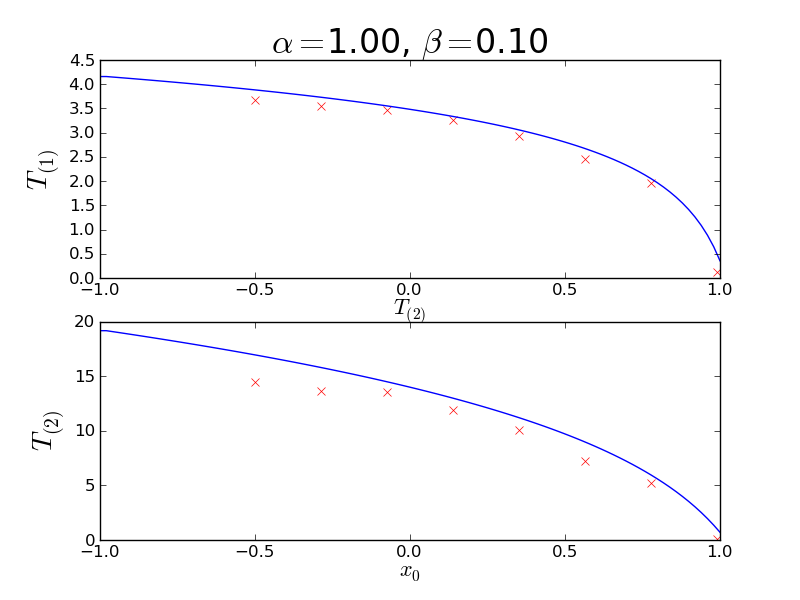
\includegraphics[width=0.48\textwidth]
{/home/alex/Workspaces/Latex/OptSpike/Figs/Moments_a=10_b=1_N=128.png}
}
\subfloat[ ]
{
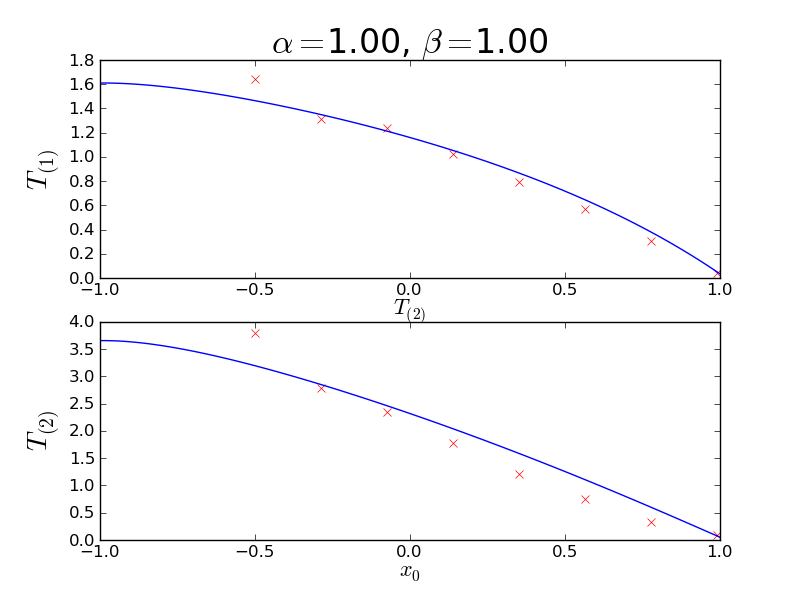
\includegraphics[width=0.48\textwidth]
{/home/alex/Workspaces/Latex/OptSpike/Figs/Moments_a=10_b=10_N=128.png}
}
\\
\subfloat[ ]
{
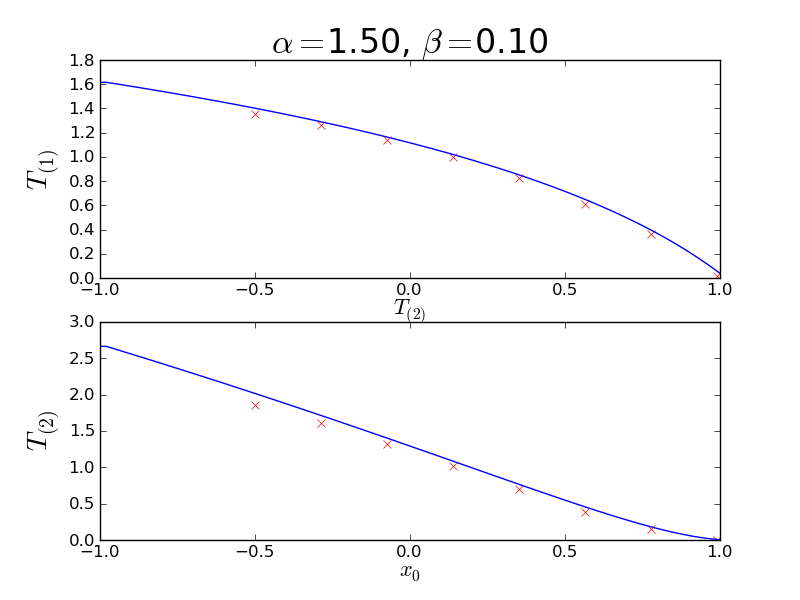
\includegraphics[width=0.48\textwidth]
{/home/alex/Workspaces/Latex/OptSpike/Figs/Moments_a=15_b=1_N=128.png}
}
\subfloat[ ]
{
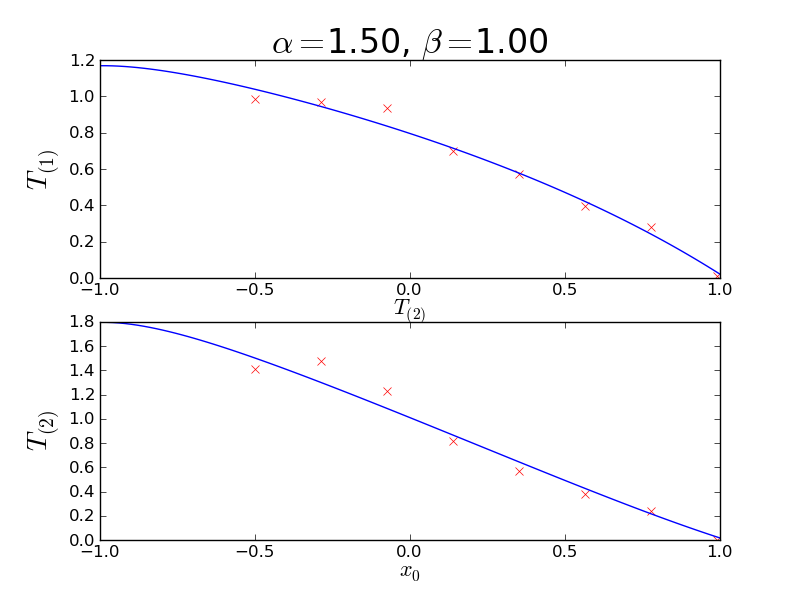
\includegraphics[width=0.48\textwidth]
{/home/alex/Workspaces/Latex/OptSpike/Figs/Moments_a=15_b=10_N=128.png}
}
\caption[]{Comparison between solutions of equations
\cref{eq:BVP_Tone,eq:BVP_Ttwo} and empirical statistics from simulating the
hitting times of \cref{eq:X_evolution_uo}. We've used only $N=128$ samples to
form the moment statistics.}
\label{fig:Ti_empirical_vs_analytic}
\end{center}
\end{figure}


\subsection{Solving the HJB}
We now have a PDE for $v$ and an algorithm for computing all the BCs and TCs of
this PDE. It is time to discuss the numerical method for solving
\cref{eq:OC_LS_HJB_full}.
Since we are in 1-d and we have the simplest geometry, the simplest thing to do
is try a centred Finite Difference scheme, upwind wherever necessary and hope
for the best. 

Things will break down if $\e$ is very small in which case the quadratic term
will dominate and cause 'havoc' or if $\b$ is very small in which case the
smoothing effect of the second derivative will be negligible and we will be in
the zone of nonlinear conservation equations. 

Let us hope for the best now and assume these two problems do not arise. 

 

\subsection{Bounded Control}
So far we have assumed that $\a$ is not constrained. However, physically, we
will have some bounds, i.e. $\a \in [\amin, \amax]$. Then the optimal control
will look like:
\begin{equation}
\astar(x,t) = \min \left(\amax, \max\left(\amin, -\frac{\di_x v}{2\e}\right)
\right)
\label{eq:OC_LS_variance_energy_quadratic_control_bounds}
\end{equation}
And the HJB becomes:
\begin{equation}
\di_t v(x,t) + \tfrac{\b^2}{2} \di_x^2 v + 
\e (\astar)^2 + (\astar-\tfrac{x}{\tc}) \di_x v 
= 0
\label{eq:OC_LS_mean_HJB_bounded_control}
\end{equation}

In the sequel we will drop the superscript $*$ on the optimal control and just
assume $\a$ is given by
\cref{eq:OC_LS_variance_energy_quadratic_control_bounds}.

\subsection{The numerical method for
\cref{eq:OC_LS_mean_HJB_bounded_control}}
 We will try the simplest thing and go from there:

Recall that we are solving backwards in time. Then for variables at the next
time-step (already computed) we will write $(\cdot)^+$; while variables at the
previous time step (to-be computed), will be denoted as$(\cdot)^-$.

Similarly given some node in space, we will write
$(\cdot)_-,(\cdot)_0,(\cdot)_+$ as the left node, the node itself and the right
node.

Then our finite-difference scheme looks like:
\begin{equation}
\frac{v^- - v^+}{\Delta t} = \tfrac{\b^2}2  .5*(\di_x^2 v^- + \di_x^2 v^+) +
(\a^+ - \tfrac{x}{\tc})  .5*(\di_x v^- + \di_x v^+) + \e (\a ^+)^2
\end{equation}

I.e. we have removed the non-linearity in $v$ by computing the control, $\a$ at
the next, already computed, time-step and used central-differencing
otherwise. We will not upwind \emph{al all} for now\ldots I.e. 
$$\di_x v = \frac{v_+ - v_-}{2\Delta x}$$
and as is standard:
$$\di_x v = \frac{v_+ - 2 v_0 + v_-}{(\Delta x)^2}$$

Will that work? Let's see - \cref{fig:HJB_attempt} shows that it works for a
particular parameter set, which sounds representative (to me). 
\begin{figure}[ht]
\begin{center}
\subfloat[Sol'n, $v$]
{
\label{fig:HJB_attempt_soln}
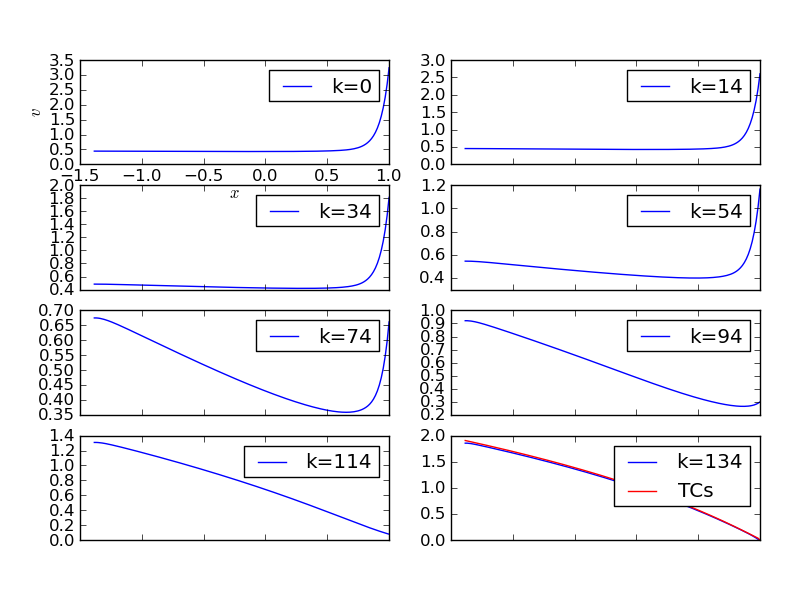
\includegraphics[width=0.48\textwidth]
{Figs/HJB/soln_al=-20_au=20__t=5_b=8.png}
}
\subfloat[Controls, $\a$]
{
\label{fig:HJB_attempt_control}
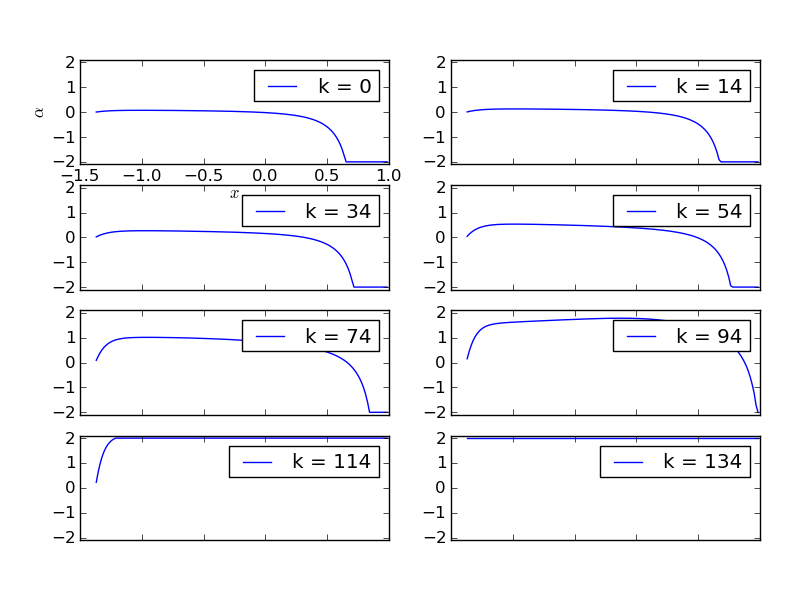
\includegraphics[width=0.48\textwidth]
{Figs/HJB/control_al=-20_au=20__t=5_b=8.png}
}
\caption[]{The solution and controls for the HJB PDE parametrized by:
$\tc = 0.50,  \beta = 0.75,
\amin = -2.00, \amax = 2.00, \eps=0.10,
\T = 1.80$. The $k$ index indicates the time-step, and recall that we are
running backwards in time, so the computation actually happens from right-to-left, bottom-to-top}
\label{fig:HJB_attempt}
\end{center}
\end{figure}
% \begin{figure}[ht]
% \begin{center}
%   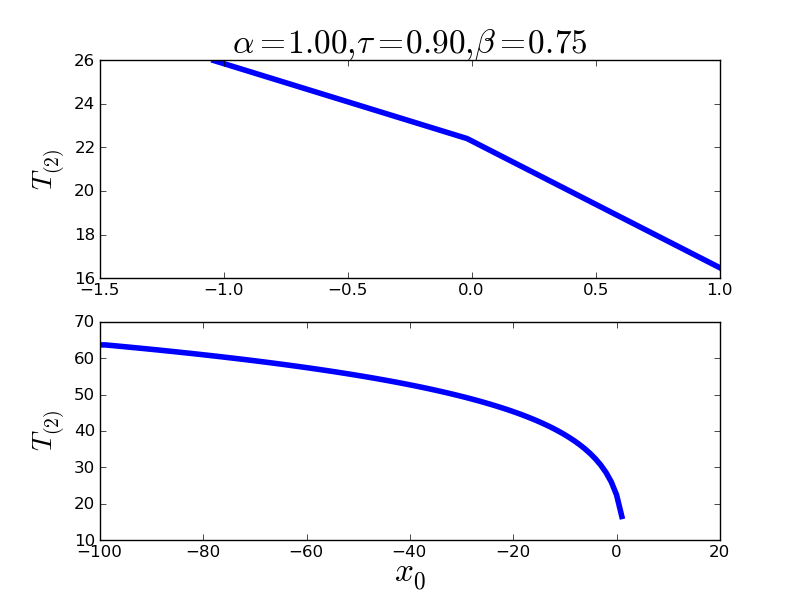
\includegraphics[width=.7\textwidth]{Figs/KolmogorovBVPMoments_a=10_t=9_b=8.png}
%   \caption[]{TCs for alpha = 1.0;  tauchar = .9; beta = .75;}
%   \label{fig:TCs_extended_x}
% \end{center}
% \end{figure}


Let's discuss the most salient features of \cref{fig:HJB_attempt}. At the end,
when $t = \T$, the value function, $v$ is monotonely decreasing. This makes
sense, becaue the lower $x$ is the more time on average will it take us to hit spike
and the more delay will we have from our desired spike time. However, as we go
back in time $v$ inverts, in the sense that for $t \ll \T$, we would like to
be somewhat far from the boundary to avoid the risk of spiking early.

Now focus on the controls, \cref{fig:HJB_attempt_control}: Naturally, at the
end we have pedal-to-the-metal type control, $\a(t>=T) = \amax$, as we start to
go back however, two things start to happen, the velocity $\a$ decreases for $x
\ll \xth$, and it even becomes negative for $x \approx \xth$. 
That is fully consistent with the problem objective - near $\xth$ and for
$t<\T$, we want to distance $X_t$ from the threshold to avoid an early spike.

So far so good. And we can be glad that for this parameter set -
there were no numerical instabilities, despite our simplistic numerical method. 

\section{Deterministic vs. Fully-Informed Stochastic Control}
At this point we are ready to attempt a comparison between a blind deterministic
type control and our stochastic control. But first let's calculate the controls
for our problem with deterministic dynamics:

\subsection{Computing the Deterministic Control}
\label{sec:deterministic_ode_control}
Since we are ignoring the noise, $\a(t)$ can be pre-calculated, for a given
$\T$. i.e. we can provide an open-loop scheme to the 'controller'.

Let's quickly derive this deterministic-case $\a$; it turns out to be very
simple:

First let's assume that we actually can get to $\xth$ from $0$ in $\T$ time
given $\amax$ and no noise. 

Then 
\begin{equation}
\begin{gathered}
J = \int_0^\T \e \a^2 \intd{t}
\\
\st
\begin{cases}
\dot{x} = (\m + \a(t) - \frac{x}{\tc})
\\
x_\T = \xth
\\
x_0 = .0
\end{cases} 
\end{gathered}
\end{equation}
The (Pontryagin) Hamiltonian becomes:
\begin{equation}
\H(x,p, \a) = \e \a^2 + p \cdot (\m + \a - x/\tc )
\end{equation}
the adjoint is given by:
\begin{equation}
-\dot{p} = \di_x \H = - p / \tc 
\end{equation} 
and the (unconstrained) control by:
\begin{equation}
\a(t) = \frac p {2 \e}
\end{equation}
which looks very similar to the stochastic case, once you put $p = \di_x v$. 

We can actually solve for the adjoint analytically: 
$$
p = p_0 \exp(t / \tc)
$$
where we can freely choose $p_0$ to later recover the TCs for $x$.
$$
\a(t) = \frac{p_0 \exp(t / \tc)}{2\e}
$$
Finally the solution for $x$ is:
\begin{align*}
\dot{x} & = \m + \a(t) -  \frac{x}{\tc}
\\ & = \m +  \frac{p_0 \exp(t / \tc)}{2\e} - \frac{x}{\tc}
\\
e^{t/\tc}x &= \int^t e^{s/\tc}\frac{p_0 \exp(s / \tc)}{2\e} \intd{s} +
				\int^t e^{s/\tc}\m \intd{s}  
\\
x &= e^{-t/\tc} \cdot \left( \frac{p_0 }{2\e} \tc \left[  e^{2 t / \tc} -1
\right] + \m\tc (e^{t/\tc} - 1)\right)
\\
&= \frac{p_0 }{\e} \tc \cdot  \sinh (t/ \tc) + \m\tc \cdot( 1 - e^{-t/\tc}))
\end{align*}
And so: 
$$
x(\T) = \xth \implies p_0 = \e \frac{ \xth - \m\tc  }{ \tc \sinh (\T/ \tc) }
$$
And we have a full solution.

If we have saturation, i.e. if $\a$ hits its bound, then the situation is mildly
more complicated. Since $p$ is monotonely increasing, as long as $p_0 >
\amin$ then $\a(t) > \amin \forall t$. So the saturation is simplified to:
\begin{equation}
\a(t) = \min \left(\frac{p_0 \exp(t / \tc)}{2\e} , \amax \right)
\label{eq:deterministic_control_bounds}
\end{equation}
In particular, $\a$ will start by following $p(t)$ and then eventually hit its
upper bound and stay there until $\T$. 

The only complication then is to calculate when $\frac{p_0 \exp(t / \tc)}{2\e} =
\amax$ and then redo the calculation for $x$ with the new control in order to
obtain the new value of $p_0$. Or we can just brute-force solve for $p_0$, by a
simple shooting method. 

using the latter approach, a solution-control pair for the parameter set we will
use later is shown in \cref{fig:deterministic_soln_controls}. 
%\usepackage{graphics} is needed for \includegraphics
\begin{figure}[htp]
\begin{center}
  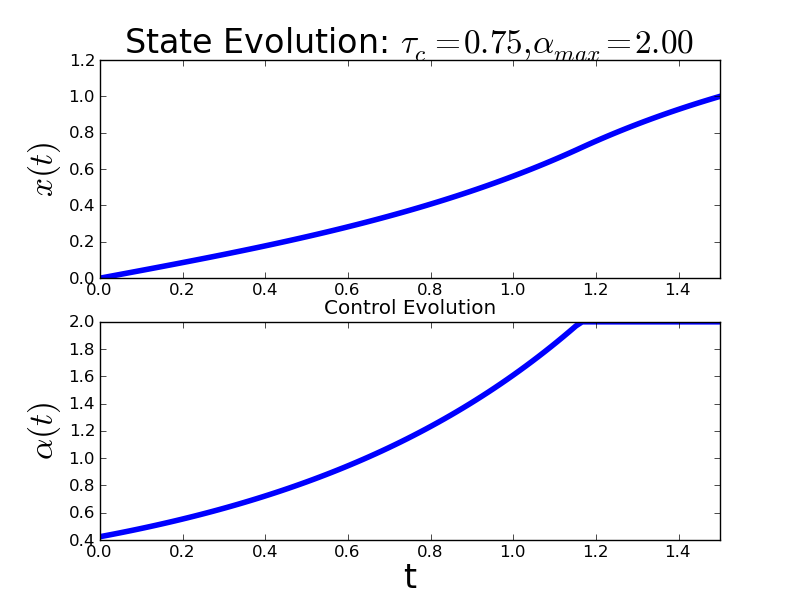
\includegraphics[width=.7\textwidth]{Figs/ControlSimulator/deterministic_example.png}
  \caption[]{An example trajectory for the deterministic dynamics. }
  \label{fig:deterministic_soln_controls}
\end{center}
\end{figure}


ALTERNATIVELY:
We can also ignore the energy cost. And just choose a constant $\a$ which will
get us to threshold at time $t=\T$. Then the calculations are:
Finally the solution for $x$ is:
\begin{align*}
\dot{x} & = \m + \a  -  \frac{x}{\tc}
\\
e^{t/\tc}x &=  \int^t e^{s/\tc}(\m+\a) \intd{s}   
\\
x &= ( \a + \m)\cdot \tc (1 - e^{-t/\tc}) 
\end{align*}
And so: 
$$
x(\T) = \xth \implies \a = \frac{\xth}{\tc(1 - e^{-\T/\tc})} - \m$$  
Assuming that $\mu$ and $\amin,\amax$ allow for a solution to this equation.
\subsection{Test Comparison}
\label{sec:deterministic_vs_feedback_numerical_test}
Let us  now make, the rather unfair, comparison of the deterministic control
against the stochastic control.

We will sample 512 realizations of the controlled system and apply either the
deterministic or the stochastic controller. Naturally, we will apply exactly
the same random disturbances to both controllers.

We will set $\e = .001$ and $\amax = 2.0$. As such the energy cost is of
secondary importance and the paramount effect on the objective is the difference
$(\ts - \T)$.
 
We show three random examples of controlled trajectories in
\cref{fig:control_trajectories_examples} and the statistical performance of the
two control laws is shown in \cref{fig:error_histograms_det_vs_stoch}. The
statistical performance of the two controllers is compared in
\cref{tab:realized_avg_errors_det_vs_stoch}. There are two important things to
note in \cref{tab:realized_avg_errors_det_vs_stoch}: first, the difference
between the deterministic-control-law and the stochastic-control-law error,
row 1 vs row 2, can be thought of as the 'added value' of feedback; second,
we see that the stochastic controller performs in practice pretty close to its
theoretical value, that is the difference between row 2 and row 3.  

The most pertinent information in 
\cref{tab:realized_avg_errors_det_vs_stoch} is that the controls we can
implement for our problem with its feedback peculiarities can never achieve a
lower error than what is achieved in rows 2,3 and should never produce a higher
error than what is in row 1.
 
\begin{table}[h] 
\centering
\begin{tabular}{lc}
Control Law & Squared Error \\
\hline
Deterministic &  0.647 \\
Stochastic &  0.336\\
Theory (Value function) & 0.285
\end{tabular}
\caption{Realized performance of the different control laws and the theoretical
expected performance of the stochastic law (last row)}
\label{tab:realized_avg_errors_det_vs_stoch}
\end{table}

\begin{figure}[h]
\begin{center}
\subfloat[A]
{
\label{fig:controlled_traj_ex1}
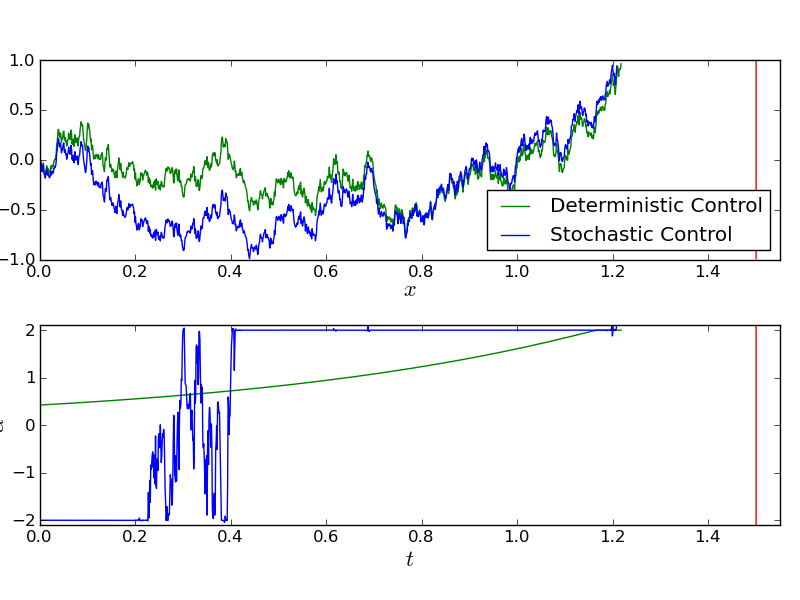
\includegraphics[width=0.33\textwidth]
{Figs/ControlSimulator/example_controlled_trajectories_id1.png}
}
\subfloat[B]
{
\label{fig:controlled_traj_ex2}
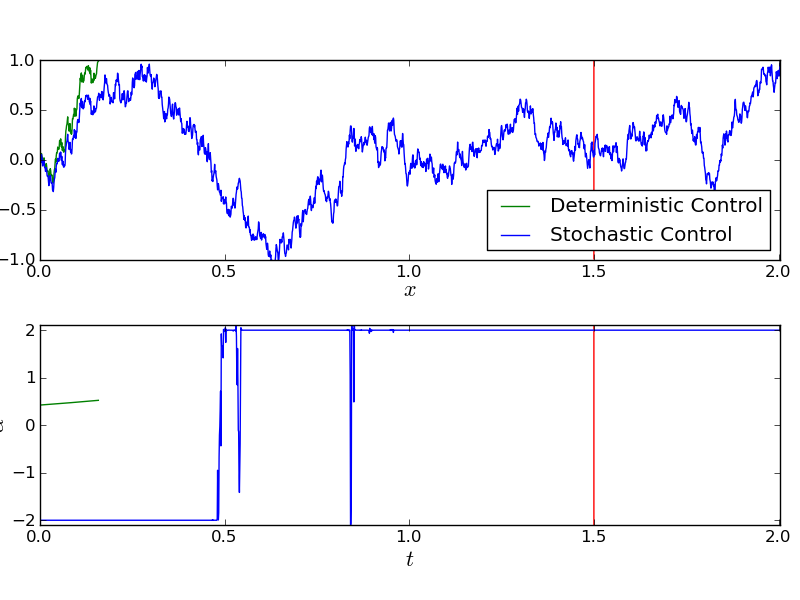
\includegraphics[width=0.33\textwidth]
{Figs/ControlSimulator/example_controlled_trajectories_id4.png}
}
\subfloat[C]
{
\label{fig:controlled_traj_ex3}
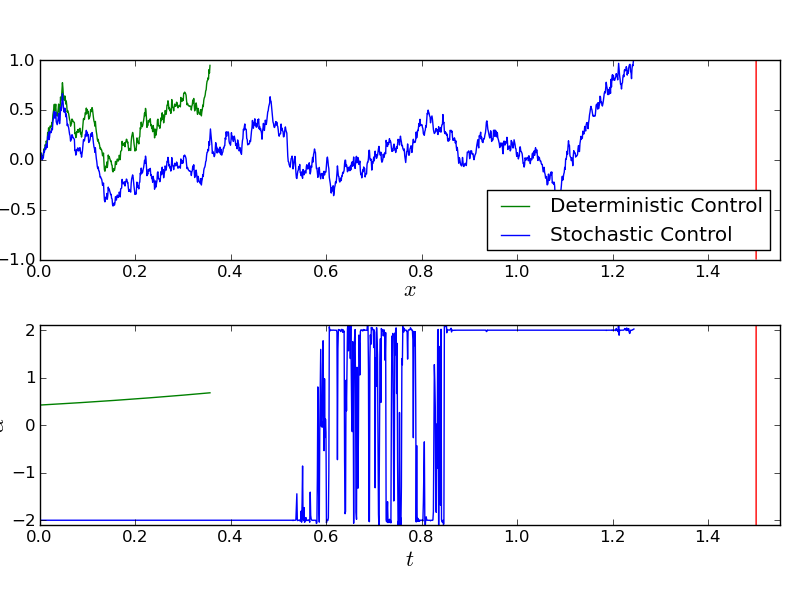
\includegraphics[width=0.33\textwidth]
{Figs/ControlSimulator/example_controlled_trajectories_id3.png}
}
\caption[]{Examples for the controlled trajectories using both the deterministic
and the stochastic control approaches. The red vertical line in the plots
indicates the desired spike-time, $\T$. In A, B the performance of both
control laws is essentially the same, but in C we see the advantage of the
stochastic approach. $\tc, \b = [.75, 1.25]$.}
\label{fig:control_trajectories_examples}
\end{center}
\end{figure}
\begin{figure}[htp]
\begin{center}
  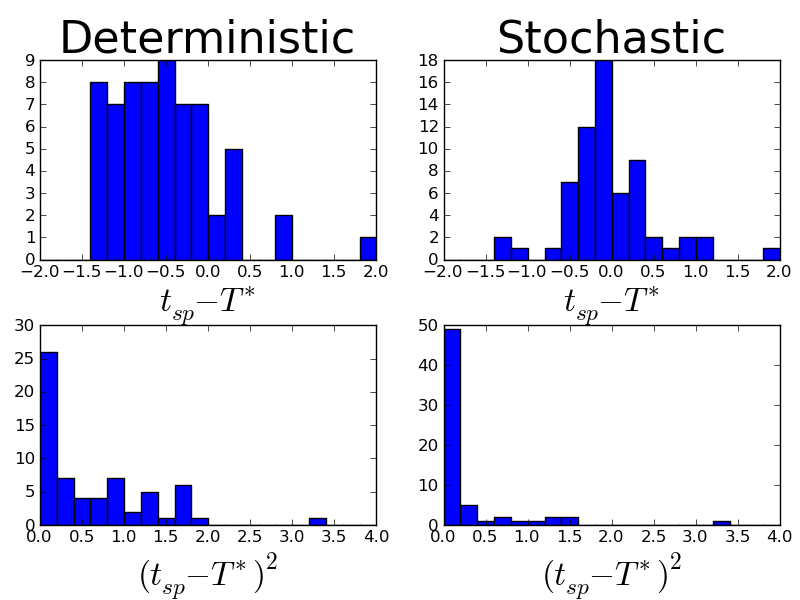
\includegraphics[width=.9\textwidth]{Figs/ControlSimulator/example_controlled_trajectories_hists.png}
  \caption[labelInTOC]{Histogram of the spike timing error for the
  deterministic (left) vs. the stochastic (right) control laws.}
  \label{fig:error_histograms_det_vs_stoch}
\end{center}
\end{figure}





\section{Uninformed Stochastic Control}
As we have mentioned before, it is unrealistic to assume we know the value of
$X_t$.

So what should we do?

Note that our main criteria - the minimization of the distance between $\ts,\T$
- is a probabilistic criterion. Since we cannot act reactively, for each
$X$ trajectory, the next most sensible thing to do is to optimize using the
transition density of $X$. We will describe how, now.

\subsection{Fokker-Plank equation for the state density evolution}
We will need the conditional transitions densities of $X$, conditional on no
spikes having occurred. We will write these as:
\begin{align*}
F(x,t) &= \Prob[X_t \leq x| X_0 = .0, X_{s<t} < \xth] &\textrm{Conditional
Dist'n}
\\
f(x,t) &= \di_x F  								   &\textrm{Conditional Density}
\end{align*}

Note that:
$$
F(\xth,t) = \int^\xth f(x,t) = \Prob[X_t \textrm{ has not spiked yet}]
$$

It is well known that for a It\^o process as in \cref{eq:X_evolution_uo},
$f$ obeys the following (forward) PDE:
\begin{equation}
\begin{gathered}
\di_t f(x,t) =
				\frac{\b^2 }{2}\cdot \di^2_x f -  
				\di_x \Big[ (\a(t)- \frac{x}{\tc})  \cdot f \Big]
\\
\\
\begin{array}{lll}
	&\textrm{st.\ }& 
	\left\{ \begin{array}{lcl}
	 f(x,0) &=& \delta(x) \quad (\textrm{delta function}
	\\
	(\a(t)- \tfrac x \tc)f - \di_x \tfrac {\b^2}2 f] \big|_{x=\xmin} &\equiv& 0
	\quad (\textrm{reflecting BCs at some } \xmin )
	\\
	f(x,t) |_{x=\xth} &\equiv& 0 \quad (\textrm{absorbing BCs at } \xth)
\end{array} \right. 
\end{array}
\label{eq:FP_pde_OU_PDF}
\end{gathered}
\end{equation}
In theory, $\xmin = -\infty$, but in the numerics below we will need to
truncate it to some finite value.

We will often encounter the probability flow term, $\phi$,:
$$
\phi(x,t) = (\a- \tfrac x \tc)f - \di_x [\tfrac {\b^2}2 f]
$$
as such the $f$ dynamics can also be written as:
$$
\di_t f(x,t) = - \di_x \phi(x,t)
$$
and the lower BC is:
$$
\phi(x,t) |_{x=\xmin} \equiv 0
$$

We will also need a short hand notation for the differential operator on the
right side of \cref{eq:FP_pde_OU_PDF}. Let
$$
\L_\a[\cdot] := \di^2_x [ \frac{\b^2 }{2} \cdot] -  
				\di_x  [ (\a(t)- \frac{x}{\tc}) \cdot]
$$
This is a linear and bounded differential operator (linearity is obvious, but
we would need to prove the boundedness) and, if we must, we will call it the
Fokker-Plank or Forward Kolmogorov differential operator. We will usually omit the
subscript $\a$, but have written it now, since the operator is parametrized by
$\a$, that is by the control.

With this, we are on our way to optimize using the density $f$ instead of a
particular trajectory $X_t$.

\subsection{Restating the objective in terms of $f$}
Let us recall our objective, \cref{eq:OC_LS_variance}:
$$
J(\a) = \Exp\left[
(\ts - \T \big)^2 
+  
\e \int_0^\ts  \a^2(s) \intd{s}
\right]
$$
Rewriting this in terms of $f$ reads:
\begin{multline}
J(\a) = 
\int_\xmin^\xth \Ttwo(x) f(x,T) \intd{x}
\\
+ \int_0^\ts \phi(\xth, s) (s-\T)^2 \intd{s}
\\
+  \e \int_0^\ts  \a^2(s)  \int_\xmin^\xth f(x,s) \intd{x} \intd{s}
\label{eq:OC_LS_variance_density}
\end{multline}

Let us explain in more detail each term on the RHS in
\cref{eq:OC_LS_variance_density}:

The first term
$$
\int_\xmin^\xth \Ttwo(x) f(x,T) \intd{x}
$$
counts the cost of trajectories which spike too late:
this cost is the expected squared time-to-hit starting at $x$, with  $\a
= \amax$, weighted by the probability of being at $x$, $f(x,T)$. Recall that we
calculated $\Ttwo(x)$ in \cref{sec:calculating_TCs}.

The second term
$$
\int_0^\ts \phi(s,t) (s-\T)^2 \intd{s}
$$
counts the cost of trajectories which spike too soon, that
is the squared difference between spike time, $t$ and desired spike time $\T$,
weighted by the probability of spike at $t$ which is just the outflow of
probability, $\phi(\xth,t)$. Note further that due to the homogeneous
Dirichlet BC on $f$ at $\xth$, the outflow is simply:
$$
\phi(\xth, t) = -\frac{\b^2 }{2} \di_x f(\xth, t) 
$$

Finally, the third term
$$
\e \int_0^\ts  \a^2(s)  \left[  \int_\xmin^\xth f(x,s) \intd{x} \right] \intd{s}
$$
is the energy cost: the inner integral, $\int_\xmin^\xth f(x,s) \intd{x}$
takes into account that we incur an energy cost only for those trajectories
which have not yet spiked.

With that our control $\a$ will naturally be found via:
$$
\a = \argmin J[\a]
$$

\subsection{Optimizing with $f$ using a Pontryagin-type Maximum Principle}
\label{sec:PDE_max_principle_for_pdf}
By now our ostensibly stochastic optimal control problem on SDEs
has become a deterministic optimal control problem on PDEs. Our control $\a$
influences the evolution density $f$ and via $f$, the integrals in the
objective, $J$.

We have already had a taste of deterministic control in
\cref{sec:deterministic_ode_control}, but the current problem is much more
complicated as it involves PDEs instead of ODEs. Thankfully we are still in 1-D
so we can solve these PDEs with simple and cheap numerical methods. 

As in the ODE theory, we will introduce a Hamiltonian functional, $\H$, and an
adjoint function, $p$, which will be crucial in setting up necessary
conditions for the optimal control.

The basic formulation for the adjoint PDEs and the abstract Hamiltonian can be
found in \cite{Fattorini1999,Palmer2011}. However our cost functional is a
little strange as it involves values of $\di_x f$ at the boundary. As such we
will 'derive' the optimality condition heuristically, appealing to the
references for rigorous proofs later.
 
Before proceeding, one might wish to read
\cref{sec:Pontryagin_heuristic_derivation} for a simpler version of the
following derivation with exactly the same ideas.

We start by assuming that $f,\a$ are the optimum trajectory/control pair and we
ask what necessary conditions must be true for $f,\a$. In particular if we take
a small variation around $\a$, we will have:
\begin{align*}
\a_\e = \a + \e \da
\\
f_\e = f + \e \df
\end{align*}

With that the variation of the cost with respect to the control at the optimal
$\a$ can be calculated as:
\begin{equation}
\frac {dJ}{d\e} \Big|_{\e = 0} =
- \int_0^\T (s-\T)^2 \frac {\b^2}{2} \di_x  \df \intd{s}  
+ \int_\xmin^\xth \Ttwo\df\intd{x}
+ \tilde{\e} \int 2 \a \da \intd{s}  
\label{eq:J_variation_PDE}
\end{equation}
This must be non-negative for a true minimum, but before we can say more, we
need to eliminate $\df$ from $\frac {dJ}{d\e}$! In order to eliminate $\df$
from \cref{eq:J_variation_PDE} we will introduce an adjoint variable, $p$. What
we would want from this adjoint variable $p$ would be that:
\begin{equation}
p(x,\T) = \Ttwo(x)
\label{eq:adjoint_TC_desideratum}
\end{equation}  
and 
\begin{equation}
\di_t [ \int_\xmin^\xth  p \cdot\df \intd{x} ] = (s-\T)^2 \frac {\b^2}{2} \di_x 
\df
 + \text{stuff}
\label{eq:adjoint_dynamics_desideratum}
\end{equation}
where 'stuff' does not depend on $\df$.

If we had such a $p$ satisfying
\cref{eq:adjoint_TC_desideratum,eq:adjoint_dynamics_desideratum} then
\cref{eq:J_variation_PDE} would read:
\begin{equation}
\frac {dJ}{d\e} \Big|_{\e = 0} =
\tilde{\e} \int 2 \a\da  \intd{s} +   \int_0^\T  \text{'stuff'}\intd{s}
\label{eq:J_variation_PDE_nodf}
\end{equation}
which does not depend on $\df$! and we'd be on our way. In order to find
$p(x,t)$ we will need to
\begin{enumerate}
  \item calculate $\di_t \df$
  \item specify $\di_t p $ st. \cref{eq:adjoint_dynamics_desideratum} holds.
\end{enumerate}

\subsection{The PDE for $\df$}
First, calculate the PDE that $\df$ satisfies:
\begin{multline}
\di_t f_\e =  \L_{\a_\e} [f_\e]
\\
= -\di_x [ (\a_\e - \tfrac{x}\tc) f_\e  - D \di_x f_\e]
\\
=  -\di_x [ (\a + \e\da - \tfrac{x}\tc) f_\e  - D \di_x f_\e]
\\
=  -\di_x [ (\a + \e\da - \tfrac{x}\tc) (f + \e \df)  - D \di_x (f + \e \df)]
\\
=  -\di_x [ (\a + \e\da - \tfrac{x}\tc) (f)  - D \di_x (f)]
- \di_x [ (\a + \e\da - \tfrac{x}\tc) (\e \df)  - D \di_x (\e \df)]
\\
= \L_\a f  -\di_x [ \e\da\cdot  f]
  +\e \L_\a \df + o(\e) 
\\
= \di_t f + \e \di_t \df
\end{multline}
Of course, we have $\di_t f = \L_\a f$, so we conclude that:
\begin{equation}
\di_t \df = \L_\a \df -\di_x [\da \cdot f] 
\end{equation}
Now what are the ICs? Well, both $f_\e$ and $f$ must satisfy the system ICs in
\cref{eq:FP_pde_OU_PDF}, so $$\df (x,0) = 0$$.
Finally, what are the BCs?
On the upper side:
$$
f_\e |_\xth = 0 = [ f  + \e \df |_\xth = 0 + \e \df|_\xth \implies \df |_\xth =
0 $$
While on the lower side:
\begin{align*}
0 =& [ (\a_\e - x/\tc)f_\e - D \di_x f_\e |_\xmin
\\
=& (\a +\e \da - x/\tc)(f + \e \df ) - D \di_x (f + \e \df) |_\xmin
\\
=& [(\a +\e \da - x/\tc)(f) - D \di_x (f) |_\xmin
\\
& + \e [ (\a +\e \da - x/\tc)(\df) - D \di_x (\df) |_\xmin
\\
=& \cancel{[(\a - x/\tc)f - D \di_x (f) |_\xmin}
\\
&+ \e \da f|_\xmin
\\
&+ \e [ (\a - x/\tc)(\df) - D \di_x (\df) |_\xmin   + o(\e)
\end{align*}
 
so $\df$ satisfies the following system of equations:
\begin{equation}
\begin{gathered}
\begin{aligned}
\di_t \df 
&= \L_\a \df -\di_x [\da \cdot f]
\\
&= -\di_x \left[ (\a - \tfrac x\tc)\df - \tfrac{\b^2}2 \di_x \df \right]
-\di_xf \cdot\da
\end{aligned}
\\
\begin{cases}
\df(x,0) &= 0
\\
[ (\a - \frac x \tc)(\df) - D \di_x (\df) |_\xmin &= -\da \cdot f|_\xmin
\\
\df|_\xth &= 0
\end{cases}
\end{gathered}
\label{eq:FP_variation_near_optimum}
\end{equation} 
With \cref{eq:FP_variation_near_optimum} we are ready to design the dynamics of
$p$ st. $\df$ is eliminated from the optimality equation,
\cref{eq:J_variation_PDE}.

\subsection{Calculating the adjoint(s)}
Recall our desideratum:
$$
p(x,\T) = \Ttwo(x) \quad (\text{required TCs})
$$
and
$$
\int_\xmin^\xth \di_t (p \cdot \df) = (s-\T)^2 \frac {\b^2}{2} \di_x 
\df + \text{stuff}
$$
Well,
\begin{align*}
\di_t (p \cdot \df) =& \df \cdot \di_t p + p \cdot   \di_t \df
 \\
 =& \df \cdot \di_t p + p \cdot \left( \L [\df] -\di_xf \cdot\da \right)  
 \\
 =& \df \cdot \di_t p + p \cdot \L  [\df] - \underbrace{ p \cdot \di_xf \cdot\da}_{\text{stuff}}
\end{align*}
Now our job is clear - we want 
$$
\di_t p = -\Lstar[p]
$$
Where $\Lstar$ is defined by:
\begin{equation}
\begin{gathered}
\int  \Lstar [p] \df \intd{x} 
=
\int p \L [\df] \intd{x} - (s-\T)^2 \frac {\b^2}{2}\di_x \df + \text{possibly
more stuff}
\\
\\
\forall \df \quad \st \begin{cases}
\df(x,t) |_{x=\xth} & = 0 
\\
(\a - \tfrac x \tc)\df - \di_x \tfrac {\b^2}2 \df \big|_{x=\xmin} &=  -\da
\cdot f
\end{cases}
\end{gathered}
\end{equation}
where 'possibly more stuff' should be independent of $\df$.

Let us take a deep breath and calculate $\Lstar$:
\begin{align*}
\int p \L [\df] \intd{x} =&
\int p (\frac{\b^2 }{2}\cdot \di^2_x \df -  
									\di_x \big[ (\a- \frac{x}{\tc})  \cdot \df \big]) \intd{x}
\\
=& [ -p ((\a- \frac{x}{\tc})  \cdot \df)\,\vert^\xth_\xmin
+ \int \di_xp ((\a- \frac{x}{\tc})  \cdot \df) \intd{x}
\\
& + [p (\frac{\b^2 }{2}\cdot \di_x \df \, \vert^\xth_\xmin 
- [ \di_x p \cdot \frac{\b^2 }{2}  \df\, \vert^\xth_\xmin 
+ \int \frac{\b^2 }{2} \di^2_xp    \cdot \df \intd{x} 
\\
=& \int \Lstar [p] \df \intd{x} 
+\underbrace{[-p(\a- \frac x \tc) \cdot \df 
+ p \frac{\b^2}{2} \di_x \df 
-\di_x p \frac{\b^2}{2} \df \, \vert^\xth_\xmin }_{\text{BC terms}}
\end{align*}

Now we want to make the 'BC terms' equal to $(s-T)^2 \frac{\b^2}{2} \di_x \df$
+ 'possibly more stuff'.
In doing so, we will discover the correct BCs associated with the adjoint
operator, $\Lstar$:
\begin{align*}
\textrm{BC terms} =& 
\Big[ -p (\a- \frac{x}{\tc})  \cdot \df 
+ p \frac{\b^2 }{2}\cdot \di_x \df   
- \di_x p \cdot \frac{\b^2 }{2}  \df   \quad ^\xth_\xmin\vert 
\\
\\
=& -\cancel{p (\a- \frac{x}{\tc})  \cdot \df \Big|_\xth}
 + p (\a- \frac{x}{\tc}) \cdot \df \Big|_\xmin
\\ 
& + [p \frac{\b^2 }{2}\cdot \di_x \df \Big|_\xth
 - [p \frac{\b^2 }{2}\cdot \di_x \df \Big|_\xmin
\\
\\
&- \cancel{[ \di_x p \cdot \frac{\b^2 }{2}   \df\Big|_\xth}
 + [ \di_x p \cdot \frac{\b^2 }{2}   \df\Big|_\xmin
\\
\\
=& \cancelto{-p (-\da f)}{-p ((\a- \tfrac x \tc)\df - \di_x \tfrac {\b^2}2
\df) \Big|_\xmin} 
+ [p \frac{\b^2 }{2}\cdot \di_x \df \Big|_\xth
+ [ \di_x p \cdot \frac{\b^2 }{2}   \df\Big|_\xmin
\\
\\
=& (s-T)^2 \frac{\b^2 }{2}\cdot \di_x \df\Big|_\xth 
+  p (\da f)\Big|_\xmin
\end{align*}

Since we want this to be true for arbitrary $\df$, we need to enforce the
following (adjoint) BCs: 
$$
\begin{cases}
p |_\xth &= (s-T)^2
\\
\di_xp |_\xmin &= 0
\end{cases}
$$

In summary, the adjoint PDE equation is given by: 
\begin{equation}
\begin{gathered}
\begin{aligned}
\di_t p =& - \Lstar[p]
\\
		=&  
			- \Big[ \frac{\b^2 }{2}\cdot \di^2_x p +  
			(\a(t)- \frac{x}{\tc})  \cdot \di_x p \Big] 
\end{aligned}
\\
\st  
\begin{cases}
	p(x,\T) &= \Ttwo(x)
	\\ 
	\di_x p  \big|_{x=\xmin} &\equiv 0
	\\
	p \big|_{x=\xth} &\equiv (s-T)^2
\end{cases}
\label{eq:adjoint_pde_OU}
\end{gathered}
\end{equation} 

And most importantly:
\begin{equation}
\int \Lstar [p] \df \intd{x}
=  
\int p \L [\df] \intd{x} 
  - (s-T)^2 \frac{\b^2 }{2}\cdot \di_x \df\Big|_\xth 
  -  p  f \cdot \da \Big|_\xmin
\label{eq:L_to_Lstar_relation}
\end{equation}

\subsection{A Pontryagin-type Minimum Principle for the optimal control $\a$}
Using \cref{eq:L_to_Lstar_relation} and the TCs in \cref{eq:adjoint_pde_OU}, we
will have:
\begin{align*}
\int \Ttwo \df \intd{x} =& 
\int_\xmin^\xth p \df \intd{x}
\\ =& \int_0^\T \di_t \int_\xmin^\xth p \cdot \df \intd{x} \intd{s}
\\
=& \int_0^\T \int _\xmin^\xth - \df \cdot \Lstar[p]
 + p \cdot \L_\a [\df] 
 -  p \cdot \di_x [\da \cdot f]  \intd{x}  \intd{s}
\\
=& 
\int_0^\T \Big\{  (s-T)^2 \frac{\b^2 }{2}\cdot \di_x \df\Big|_\xth 
+  p (\da f)\Big|_\xmin
\\
& \quad
- \int _\xmin^\xth p \cdot \di_x [\da \cdot f] \intd{x} \Big\} \intd{s}
\end{align*}

Now put this back into the equation of optimality, \cref{eq:J_variation_PDE}.
\begin{align*}
\frac {dJ}{d\e} \Big|_{\e = 0} =&
- \int_0^\T (s-\T)^2 \frac {\b^2}{2} \di_x  \df \intd{s}  
+ \int_\xmin^\xth \Ttwo\df\intd{x}
+ \tilde{\e} \int 2 \a \da \intd{s}
\\
=& 
\int_0^\T \Big\{
 p (\da f)\Big|_\xmin
+ \tilde{\e}  2 \a \da
- \int _\xmin^\xth p \cdot \di_x [\da \cdot f] \intd{x} 
 \Big\} \intd{s}
 \\
=& 
\int_0^\T \da \Big\{
 p f \Big|_\xmin
+ \tilde{\e}  2 \a
- \int _\xmin^\xth p \cdot \di_x f \intd{x} 
 \Big\} \intd{s}
\end{align*}

Now we pull the famous fundamental lemma of the calculus of variations out and
conclude that
\begin{equation}
\Big\{
 \tilde{\e}  2 \a(t)
+ p f \Big|_\xmin
- \int _\xmin^\xth p \cdot \di_x f \intd{x} 
\Big\} = 0
\quad \forall t \in [0,T]
\label{eq:J_necessary_condition}
\end{equation}

Working in reverse we can recognize a Hamiltonian, $\H$ as:
$$
\H(f,p,\a) =  \int \cref{eq:J_necessary_condition} \intd{\a} 
$$

Naturally, $f,p$ must satisfy their respective
\cref{eq:FP_pde_OU_PDF,eq:adjoint_pde_OU}.

And our optimal control, $\a$,  can be found via:
\begin{equation}
\a (t) = \frac { - p(\xmin,t) f(\xmin,t)
+ \int _\xmin^\xth p(x,t) \cdot \di_x f(x,t) \intd{x} 
}{2\e}
\label{eq:optimal_alpha_4_PDF_optimization}
\end{equation}
As always, subject to the appropriate bounds, \cref{eq:bound_constraints_alpha}.

\subsection{An Iterative Numerical Solution}
We have an entangled situation: $f,p$ depend on $\a$, but $\a$, the optimal
control, is given by the solution to $f,p$. So we need some kind of iteration to
find $\a$ and the corresponding $f,p$.

The key to such an iteration is that the quantity, 
$$\di_\a \H =  \Big\{
 \tilde{\e}  2 \a(t)
+ p(x,t) f(x,t) \Big|_\xmin
- \int _\xmin^\xth p \cdot \di_x f(x,t) \intd{x} 
\Big\}
$$ gives us the direction of increase
and we can use it as a gradient in a descent algorithm. 
This we can also write as:
\begin{align*}
\di_\a \H =&  \Big\{
 \tilde{\e}  2 \a(t)
+ p(x,t) f(x,t) \Big|_\xmin
- [p(x,t) f(x,t) \, _\xmin^\xth\Big|
+ \int _\xmin^\xth \di_x p \cdot f(x,t) \intd{x} 
\Big\}
\\
=&
 \Big\{
 \tilde{\e}  2 \a(t)
- p(x,t) f(x,t)\Big|_\xth
+ 2p(x,t) f(x,t) \Big|_\xmin
+ \int _\xmin^\xth \di_x p \cdot f(x,t) \intd{x} 
\Big\}
\end{align*}
which has certain numerical advantages.



So the plan is: we choose an initial $\a_1(t)$ - the deterministic solution
from \cref{sec:deterministic_ode_control} is a natural choice. Then solve for $f,p$.
Then evaluate $J$ and iterate until convergence. (Until $J$ stops getting smaller.)

More specifically see the pseudo-code in
Algorithm \ref{alg:hamiltonian_descent_4_PDF_OC}:
\begin{algorithm}
\begin{algorithmic}
\State $J_0 = \infty $ 
\State $\a_1 = $ Deterministic $\a$
\For { $k= 1\dots k_{\max}$}
	\State $\di_t f_{k} = \L_{a_{k}} [ f_{k}]$
	\State $-\di_t p_{k} = \Lstar_{a_{k}} [ p_{k}]$
	\State $J_{k} \gets J[\a_k, f_k]$
	\If {$|J_{k} - J_{k-1}| < tol $}
		\State BREAK
	\EndIf
	\State $\da = \di_a \H(f_{k} ,p_{k},  \a_{k})$

	\If {$\sup_t |\da(t)| < tol$}
		\State BREAK
	\EndIf

	\State $\a_{k+1} \gets \a_{k} - s \cdot \da  $
\EndFor
\State \Return $J_k, \a_k$
\end{algorithmic}
\caption{Optimal Control Descent Algorithm}
\label{alg:hamiltonian_descent_4_PDF_OC}
\end{algorithm}


We show one realization of $\di_a \H$ in \cref{fig:grad_aH_deterministic_alpha}.
Also, we can calculate $J$ for the deterministic $\a(t)$. We find it is
$J[\a_{\text{det}}] = .709$, which is quite close to the experimentally observed
$J$ in the first row of \cref{tab:realized_avg_errors_det_vs_stoch} and so we
know we are on the right path.
%\usepackage{graphics} is needed for \includegraphics
\begin{figure}[htp]
\begin{center}
\subfloat[$\a_0$]
{
  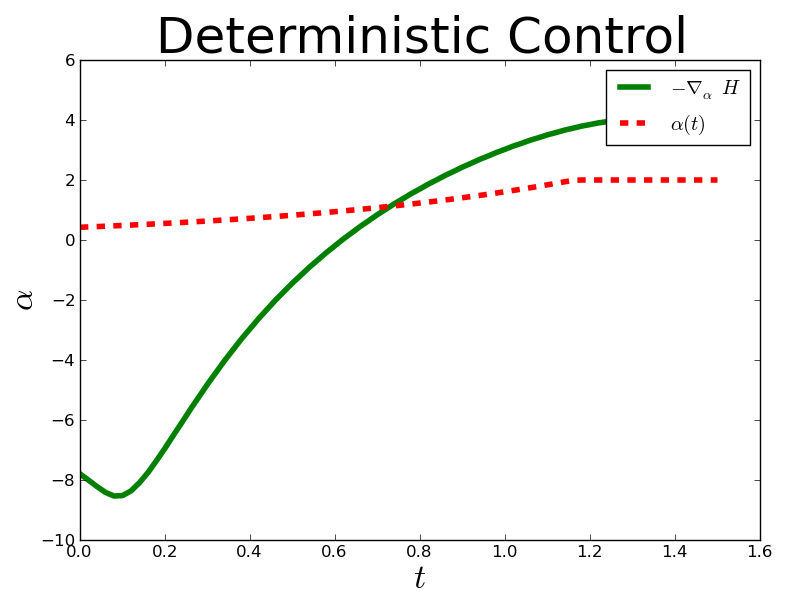
\includegraphics[width=.49\textwidth]{Figs/FP_Adjoint/Deterministic_alpha_di_aH.png}
  }
  \subfloat[$\a_1$]
{
  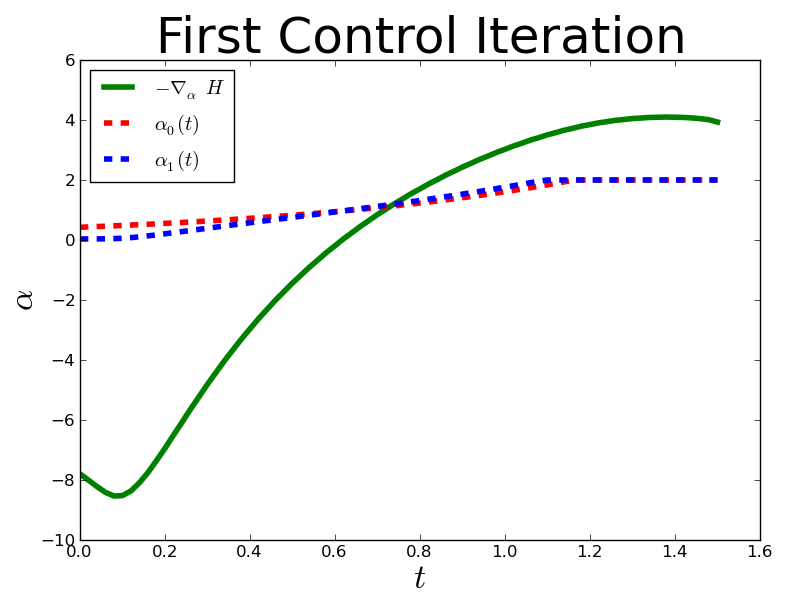
\includegraphics[width=.49\textwidth]{Figs/FP_Adjoint/First_control_iteration.png}
  }
  \caption[labelInTOC]{Example of $-\di_a \H$ calculated at $\a(t)$ being the
  deterministic control, the information is that we need to decrease $\a$ at the beginning and increase it
  towards the end (if possible due to the bound) and the resulting incremental
  change, $\a_1$, is shown on the right. }
  \label{fig:grad_aH_deterministic_alpha}
\end{center}
\end{figure} 


Finally, we are ready to calculate the open-loop, stochastic optimal control
(for this parameter set) - the results are in
\cref{fig:FP_adjoint_objective_control_convergence}. We see that all our work
was not for naught:-)

\begin{figure}[h]
\begin{center}
\subfloat[$\a_k(t)$ ]
{
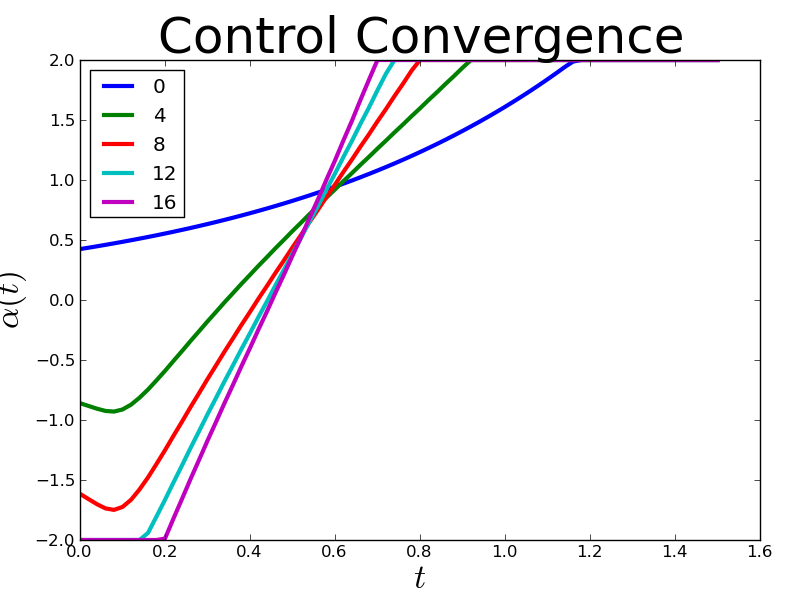
\includegraphics[width=0.48\textwidth]
{Figs/FP_Adjoint/ExampleControlConvergence_control.png}
}
\subfloat[$J_k$ ]
{
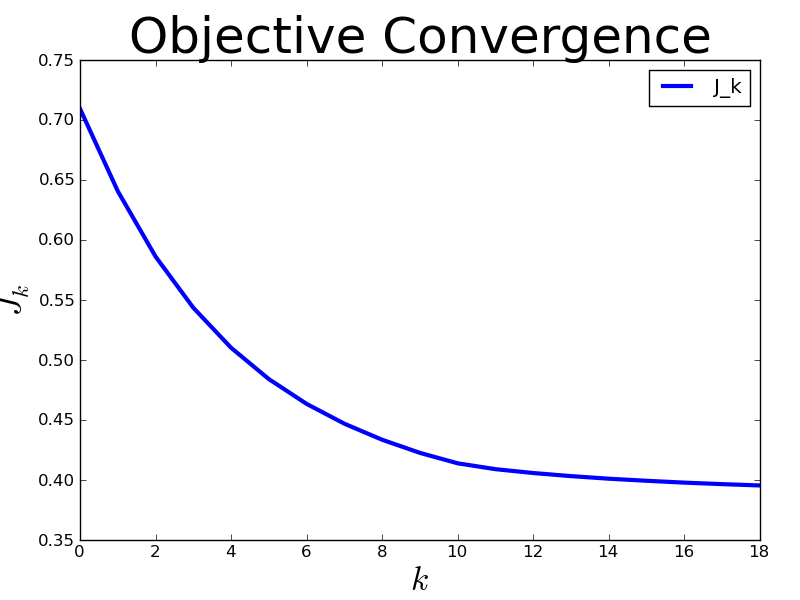
\includegraphics[width=0.48\textwidth]
{Figs/FP_Adjoint/ExampleControlConvergence_objective.png}
}
\caption[ ]{The result of an optimization iteration, on the left the various
controls, on the right the progress of the objective. THe final control is much
more inhibitory at the beginning, than the deterministic control. Moreover, we
see that there is a significant improvement in the objective (about 43\%)}
\label{fig:FP_adjoint_objective_control_convergence}
\end{center}
\end{figure}


\subsection{Test Comparison}
\label{sec:probabilistic_numerical_test}
We will now run our open-loop stochastic control obtained in \cref{fig:FP_adjoint_objective_control_convergence}
through the same comparison test as we did for the deterministic open-loop control and the stochastic
feedback (closed-loop) control in
\cref{sec:deterministic_vs_feedback_numerical_test}, with the same parameter
values, $\e, \T, \amax, \beta, \tc$. From
\cref{fig:FP_adjoint_objective_control_convergence}, we expect that our
open-loop control should do quite better than the deterministic control, and not
too much worse than the feedback stochastic control - let us see if that is
indeed the case. As before we report the gross results in
\cref{tab:realized_avg_errors_det_vs_openloop_vs_stoch}, show the error
histograms in \cref{fig:error_histograms_det_vs_openloop_vs_stoch} and
visualize some trajectories in
\cref{fig:control_trajectories_examples_with_openloop}. 

The basic conclusion is that it was all worth it! The open-loop stochastic
control is certainly not as good as the feedback stochastic control, but it is much closer in performance to
it, than to the blind deterministic control. 

\begin{table}[h] 
\centering
\begin{tabular}{lc}
Control Law & Squared Error \\
\hline
Deterministic &  0.621 \\
Open-Loop Stochastic & 0.356 \\
Feedback Stochastic &  0.288\\
\hline
Openloop Theory (J) & 0.382
\\
Feedback Theory (Value function) & 0.285
\end{tabular}
\caption{Realized performance of the different control laws and the theoretical
expected performance for the stochastic laws (last 2 rows)}
\label{tab:realized_avg_errors_det_vs_openloop_vs_stoch}
\end{table}
\begin{figure}[h]
\begin{center}
\subfloat[A]
{
\label{fig:controlled_traj_ex1}
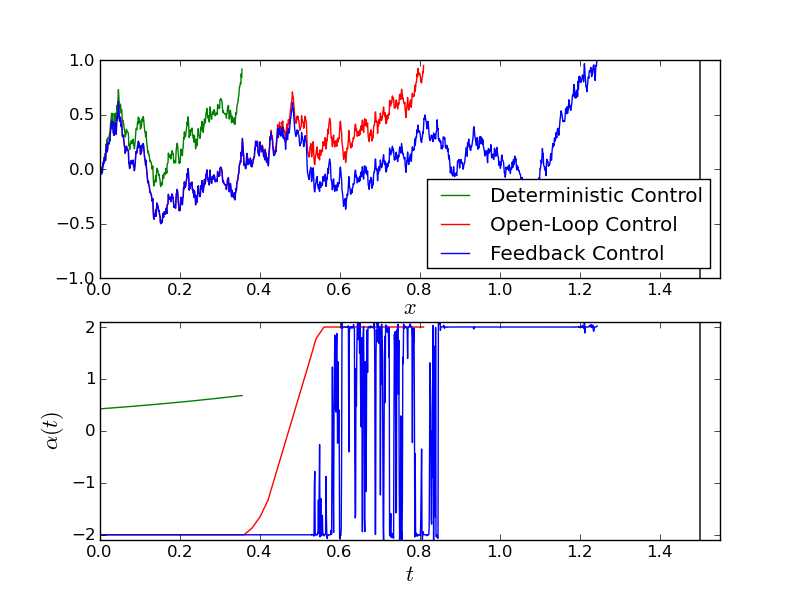
\includegraphics[width=0.33\textwidth]
{Figs/ControlSimulator/3controls_example_trajectories_id3.png}
}
\subfloat[B]
{
\label{fig:controlled_traj_ex2}
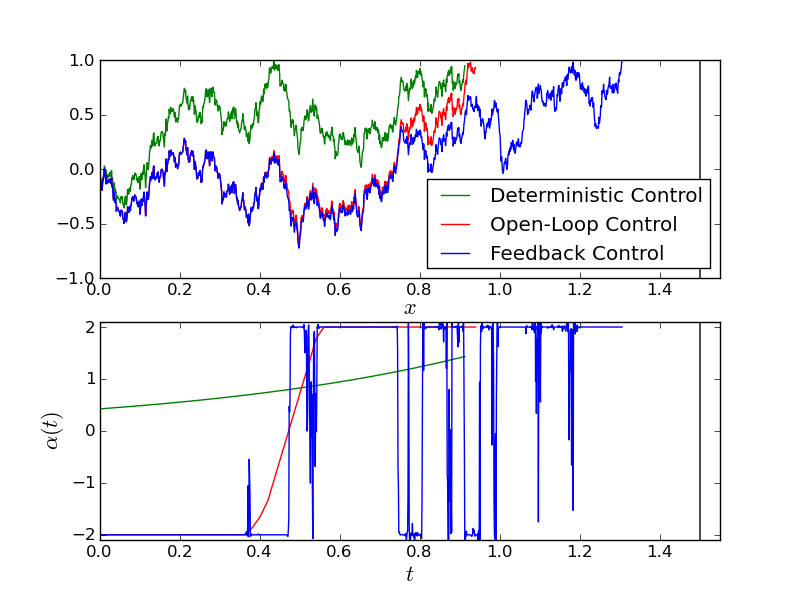
\includegraphics[width=0.33\textwidth]
{Figs/ControlSimulator/3controls_example_trajectories_id5.png}
}
\subfloat[C]
{
\label{fig:controlled_traj_ex3}
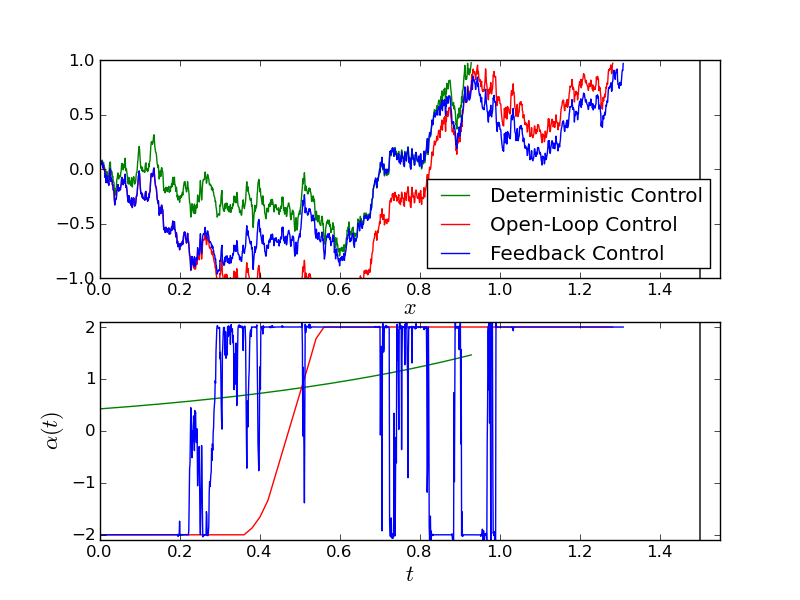
\includegraphics[width=0.33\textwidth]
{Figs/ControlSimulator/3controls_example_trajectories_id6.png}
}
\caption[]{Examples for the controlled trajectories using the deterministic,
open-loop stochastic and feedback stochastic control approaches. The
black vertical line in the plots indicates the desired spike-time, $\T$. $\tc,
\b = [.75, 1.25]$.}
\label{fig:control_trajectories_examples_with_openloop}
\end{center}
\end{figure}

\begin{figure}[h]
\begin{center}
  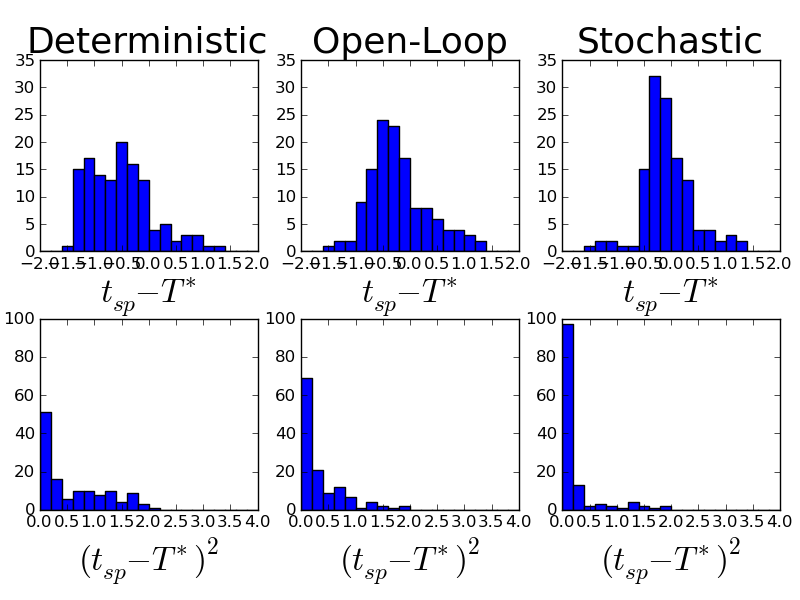
\includegraphics[width=.95\textwidth]
  {Figs/ControlSimulator/3controls_example_trajectories_hists.png}
  \caption[labelInTOC]{Histogram of the spike timing error for the
  deterministic (left) vs. open-loop stochastic(centre) vs. feedback stochastic
  (right) control laws. $N=128$}
  \label{fig:error_histograms_det_vs_openloop_vs_stoch} 
\end{center}
\end{figure}

% \subsection{Optimizing with $f$ - the Direct Approach}
% The adjoint approach to optimizing with PDEs is actually more appropriate when
% we have a distributed control\ldots
% 
% Here we have a much more crude single-variable control - the value of $\a$ at a
% given time. So it might be simpler to just apply the direct approach of Optimal
% Control and discretize the system and converge to the minimum. We have not
% explored this for now.

\newpage
% \section{Hacked reuse of the HJB control}
% A more simple-minded approach is to use the HJB controller with an estimate,
% $\xest$, for the state. Since there are no observations, the only sensible
% estimate would be the mean of the process. 
% We will write 
% \begin{align*}
% \mcond &= \Exp [X_t | X_{s<t} < \xth] = \int x f(x,t)
% \intd{x} &(\textrm{Conditional Mean})
% \end{align*}
% then 
% \begin{align*}
% \Exp[X_t | X_{s<t} < \xth] &= \frac{\int_\xmin^\xth x \di_xF(x) \intd{x} }{
% \int_\xmin^\xth  \di_xF(x) \intd{x}}
% \\
% &= \frac{[x F(x) |_\xmin^\xth \quad - \quad \int_\xmin^\xth  F(x) \intd{x} }{
% F(x) |_\xmin^\xth}
% \\
% &= \xth - \frac{\int_\xmin^\xth  F(x) \intd{x}} {F(\xth)}
% \\
% &= \mcond
% \end{align*}
% For a consistency check, note that $\xest = .0$ at $t = 0$, since
% $F(\xth,0) = 1.$ and $\int_\xmin^\xth H(x) \intd{x} = \xth$, as long as $\xmin <.0$, which it is.

\section{Sample-based solution to Open-Loop control}
In the previous section we have set up and numerically solved a
state-adjoint pair of PDEs which helps us find the Optimal Control using
a simple and efficient gradient-based iterative scheme.

We now discuss how to perform the solution using trajectory samples instead of
numericallly solving a pair of PDEs. To this end we will use the Feynman-Kac
formula, once we realize that the adjoint PDE has a Feynman-Kac representation.  

\subsection{Fokker-Planck and Feynman-Kac}
We know that the solution to the forward PDE for $f(x,t)$,
\cref{eq:FP_pde_OU_PDF} represents the density of samples at $(x,t)$
that start from $x=0$ at $t= 0$. 
$$
f(x,t) = \Prob[ X_t = x| X_0 = 0]
$$

What is less obvious is that the adjoint PDE
for $p(x,t)$, \cref{eq:adjoint_pde_OU}, has the following stochastic
representation:
\begin{align}
p(x,t) =&
	\Exp\Big[(\ts - \tf)^2 + \e\int_0^\tf u(s) \intd{s} \,|\, X_t = x \text{
	AND } \ts \leq \tf \Big] \notag
\\ 	\,	&
	\Exp \Big[\Ttwo(X_\tf) + \e\int_0^\ts u(s) \intd{s} \,|\, X_t = x \text{ AND }
	\ts> \tf \Big] +\,
\label{eq:adjoint_FeynmanKac_representation}
\end{align}
i.e. $p(x,t)$ gives the expected cost of a trajectory that goes through $x$ at
time $t$.

Recall that we need $f,p$ in order to calculate the gradient:
$$\di_\a \H =  \Big\{
 \tilde{\e}  2 \a(t)
+ p(x,t) f(x,t) \Big|_\xmin
- \int _\xmin^\xth p \cdot \di_x f(x,t) \intd{x} 
\Big\}
$$
If we use samples, we do not need to artificially truncate the domain from below
so we can drop the $p(x,t) f(x,t) \Big|_\xmin$ term. And we just need to
calculate either:
$$ - \int_{x < \xth} p(x,t) \cdot \di_x f(x,t) \intd{x}$$
or, equivalently, by integrating-by-parts:
$$   \int_{x < \xth} \di_x p(x,t) \cdot f(x,t) \intd{x}$$
If we sample then this is just an expectation with respect to $X$ and can be
written as: 
\begin{equation}
\int_{x < \xth} \di_x p(x,t) \cdot f(x,t) \intd{x} = \Exp[\di_x p(X,t) ]
\approx 1/N\sum_i \di_x p(X^{(i)}_t,t) 
\label{eq:f_sampled_vs_f_solved}
\end{equation}   
where $\{ X^{(i)}_t \}_{i=1}^N$ are the samples. This expression would be
particularly useful if we had a closed form expression for $\di_x p$, but that
is usually not the case.

We show a comparison of the two ways of computing
\cref{eq:f_sampled_vs_f_solved} simulation vs. PDE in
\cref{fig:f_sampled_vs_f_solved}. We see a ball-park agreement and of course,
the simulation-based approximation is noisy.
% \usepackage{graphics} is needed for \includegraphics
\begin{figure}[htp]
\begin{center}
  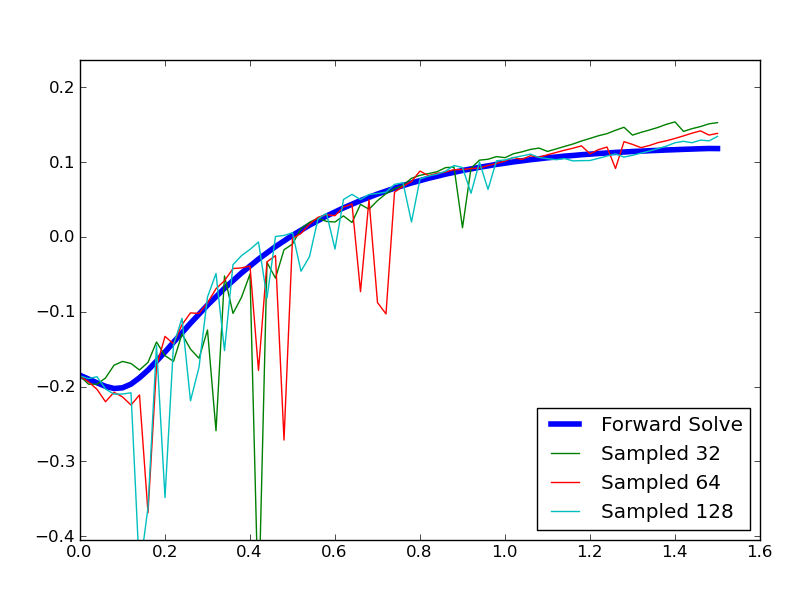
\includegraphics[width=.9\textwidth]{Figs/FeynmanKac/fsampled_psolved_t=8_b=12.png}
  \caption{Simulation vs.\ the PDE mode of computing $\di_\a \H$.
  Recall $p$ is solved using PDE numerics, but $f$ is simulated using trajectory
  samples. Thus, $\int \di_x p f $ at time $t$ is approximated as $1/N
  \sum_{X_t < 1} \di_x p(X_t)$.}
  \label{fig:f_sampled_vs_f_solved}
\end{center}
\end{figure}

If we would like to dispense with solving for $p$ as well then we need a way to
compute $\di_x p$ from the samples. As we said, the Feynman-Kac formula gives us
a stochastic representation for the solution of a PDE. But we need the
partial derivative of that solution with respect to $x_t$\ldots It's not obvious
what to do, we can obtain a PDE for $\psi = \di_x p$, by just differentiating
the $p$ PDE and that will give us a Feynman-Kac type evolution, but we don't
know the right BCs. We would know the TCs: $\psi(\tf) = \di_x \Ttwo(x)$, but we
don't know what to do at the threshold boundary $x=\xth$\ldots and using a
finite difference approximation would be proxibitive, b/c then for every point
in space-time we would need to start a bunch of simulations. Maybe we shold go
back to trying to evaluate $\int \di_x f \cdot p$ and look for sample-based
approximations of $\di_x f$?


\section{Spike Response Model}
An alternative model to the hard-threshold LIF model is the Spike Response
Model. The difference is that here a neuron spikes with instantaneous rate
$\lambda$:
where usually
$$
\lambda(x) \propto exp(x)  
$$
that is, we want $\lim_{-\inf} \l = 0$ and $\lim_{\inf} \l = \infty$, meaning
that for very low voltages spikes are impossible and for very  high voltages,
spikes are inevitable and instantaneous. 

With this the Fokker-Planck PDE becomes:

\begin{equation}
\begin{gathered}
\di_t f(x,t) =
				\frac{\b^2 }{2}\cdot \di^2_x f -  
				\di_x \Big[ (\a(t)- \frac{x}{\tc})  \cdot f \Big]
				-\l(x) f 
\\
\\
\begin{array}{lll}
	&\textrm{st.\ }& 
	\left\{ \begin{array}{lcl}
	 f(x,0) &=& \delta(x) \quad (\textrm{delta function}
	\\
	(\a(t)- \tfrac x \tc)f - \di_x \tfrac {\b^2}2 f] \big|_{x=\xmin} &\equiv& 0
	\quad (\textrm{reflecting BCs at some } \xmin )
	\\
	(\a(t)- \tfrac x \tc)f - \di_x \tfrac {\b^2}2 f] \big|_{x=\xmax} &\equiv& 0
	\quad (\textrm{reflecting BCs at some } \xmax )
\end{array} \right. 
\end{array}
\label{eq:FP_pde_OU_PDF_SRM}
\end{gathered}
\end{equation}
The biggest difference between \cref{eq:FP_pde_OU_PDF_SRM} and
\cref{eq:FP_pde_OU_PDF} is the addition of the killing term $-\l f$ and the
different domain and boundary conditions.  For the Spike Response Model, we need
a bigger domain, since the voltage can become arbitrary high, but the decay term
will pull it back towards $\a$, meaning by symmetry we should have $\xmax +
\xmin = 2\alpha$.

Now spikes happen throughout the domain (with frequency $\l f$) and thus the
objective function $
J(\a) = \Exp\left[
(\ts - \T)^2 + \e \int_0^\ts  \a^2(s) \intd{s}
\right]
$ in terms of $f$ now reads:
\begin{align}
J(\a) = &
\int_\xmin^\xmax \Ttwol(x) f(x,T) \intd{x}
\\
&+ \int_0^\ts (s-\T)^2  \int_\xmin^\xmax \l(x) f(x,s) \intd{x}\intd{s}
\notag
\\
&+  \e \int_0^\ts  \a^2(s)  \int_\xmin^\xmax f(x,s) \intd{x} \intd{s}
\notag
\label{eq:OC_LS_variance_density_SRM}
\end{align}
here we have $\Ttwol(x)$ as the squared time to spike in the soft-threshold
framework starting at $x$. This is, of course, different from $\Ttwo(x)$
which is the squared time to spike in the hard-threshold model.

In fact one can see that the soft-threshold includes the hard-threshold in the
special case that $\l(x) = \delta (x-\xth)$.

\subsection{Calculating  $\Ttwol(x)$}
OMIT FOR NOW, assume it can be dones as easily as $\Ttwo(x)$.

\subsection{The SRM Adjoint}
We will skip deriving the BCs for the adjoint $p$ and just state the PDE:
\begin{equation}
\begin{gathered}
\begin{aligned}
\di_t p(x,t) =& - [ \Lstar[p] + (s-\T)^2 \l(x) ]   
\\
		=&  
			-\Big[ \frac{\b^2 }{2}\cdot \di^2_x p +  
				(\a(t)- \frac{x}{\tc})  \cdot \di_x p 
				- \l(x) p
				+ (s-\T)^2 \l(x) 
			\Big] 
\end{aligned}
\\
\st  
\begin{cases}
	p(x,\T) &= \Ttwol(x)
	\\ 
	??? \di_x p  \big|_{x=\xmin} &\equiv 0 ???
	\\
	??? \di_x p  \big|_{x=\xmin} &\equiv 0 ???
\end{cases}
\label{eq:adjoint_pde_OU_SRM}
\end{gathered}
\end{equation} 

Optimal principles and objective gradients follow exactly as before:

\subsection{Feynman-Kac for the SRM Model}
Recall the difficulty we had with the hard-threshold model and implementing the
Feynman-Kac formula. In particular, since we needed the value of $\di_x p =:
\psi$ we were stuck. 

However, with the soft-threshold formula we have:
$$
\di_x \di_t p(x,t) = 
			-\di_x \Big[ \frac{\b^2 }{2}\cdot \di^2_x p +  
				(\a(t)- \frac{x}{\tc})  \cdot \di_x p 
				- \l(x) p
				+ (s-\T)^2 \l(x) 
			\Big] 
$$
so $\psi = \di_x p$ obeys the following F-K type equation:
$$
\di_t \psi  
+ \frac{\b^2 }{2} \di^2_x \psi 
+ \left(\a(t)- \frac{x}{\tc}\right) \di_x \psi
- \frac{1}{\tc}    \psi
-  \l(x) \psi
- \boxed{\l'(x) p}
+ (s-\T)^2 \l'(x)
= 0
$$
Ooops! We still have a $p$ term in there, which we have to calculate
separately\ldots but we can do that again with a F-K type expectation. For the
$\psi$  TCs, we have:
$$
 \psi(\tf) = \di_x \Ttwol(x)
$$
 Let us rewrite the PDE for $\psi $ in a standard form:
 $$
 \di_t \psi  
 +  U(x,t) \di_x \psi 
 +  D(x,t) \di^2_x \psi
 - \underbrace{V(x,t)}_{ 1 / \tc + \l(x)} \psi 
 + \underbrace{f(x,t)}_{( (s-\T)^2  - p) \l'(x)} = 0
 $$
  
% $$
% \di_t p(x,t) + \Big[ \frac{\b^2 }{2}\cdot \di^2_x p +  
% 				(\a(t)- \frac{x}{\tc})  \cdot \di_x p 
% 				- \l(x) p
% 				+ (s-\T)^2 \l(x) 
% 			\Big] = 0
% 			$$
then we can evaluate $\psi$ as conditional expectations\footnote{I need a
better reference than: WP \url{http://en.wikipedia.org/wiki/Feynman-Kac_formula}}:
$$
\psi(x,t) = 
\Exp \left[
\int_t^\tf  f(X_s, s) e^{-\int_t^sV(X_\t,\t) \intd{\t}}
\intd{s}
+
e^{-\int_t^\tf V(X_\t,\t) \intd{\t}} \psi(X_\tf)) | X_t = x
\right] $$ 
where the expectation is done over the RV $X_t$  with the dynamics: $$
dX = U(x,t)dt + \sqrt{2D} \intd{W}
$$
which are exactly the same dynamics as the ones for the forward process. This
means that the same trajectory can be used to compute both the distribution $f$
and the adjoint and its derivative $p$ and $\psi$. 
This means that we can perform a simulation for $X$ and then unroll the
calculation backwards to obtain $p, \psi$ and 
$\int_x f(x,t) \di_x p(x,t) \intd{x} \approx \sum_i \psi(X_t^{(i)} )$

% \section{Refractoriness}
% Our models have so far not included an expl
\section{The multivariate case}
Our methods are only worth anything if we can scale them to the multivariate and
indeed to the massive multivariate case, with more than 10 neurons, i.e\
states. This makes the direct pde approach very difficult, since a PDE 


\section{The Big Questions}
Where are we going with all this? 

So far, we have a cleanly set-up problem. It has been numerically solved for a
limited range of parameters and there is no obvious difficulty in extending the
solution scheme to the entire relevant parameter range. A curious challenge
would be to what extent the implementation can be pushed to be 'real-time',
i.e.\ whether this optimization can be done online with neurons spiking at
frequencies on the order of 20-50 kHz (inter-spike intervals of 20-50 ms.), at
least in {\sl silico}.

A much more ambitious goal is to see whether this can be done for many neurons
(say $N=25$) which have coupled control/dynamics. This is very challenging,
because a naive application of most of the techniques used so far will result in
us having to solve a 25-dimensional PDE and that is essentially
impossible\footnote{with 10 nodes discretizing each neuron state we will need
$10^{16}$ Gbytes to store one time-step of $v$ so, for one, we won't have enough
memory}. Thus PDE methods cannot be directly applied and either some kind of
independence between the neurons needs to be assumed or a different control
technique should be applied - perhaps, and very speculatively, a path-integral
control approach as in \cite{Kappen2007,Theodoru2011}.

Note that $N=26$ was accomplished in \cite{Ahmadian2011}, but they used a
different spiking model, which allowed for certain analytical tricks to greatly
simplify the mathematics. Perhaps a conclusion that will come out of this whole
research is that one should use their models (known as Spike Response
Models) and not the hard-threshold LIF model if one wants to do optimal control
over spike trains. 

We don't know until we try.

% \begin{quote}
% \raggedleft
% Life can only be understood backwards; but it must be lived forwards.
% \\
% \textsl{Soren Kierkegaard}
% \end{quote}

\newpage
\appendix
\section{Heuristic Derivation of Pontryagin's Minimum Principle}
\label{sec:Pontryagin_heuristic_derivation}
Here we will show a heuristic derivation for the Pontryagin Minimum Principle
for linear ODE dynamics. It should motivate the manipulations in
\cref{sec:PDE_max_principle_for_pdf}.

The following is almost a direct transcription A.1 in
\cite{Evansb}, with the added simplification of linear dynamics
and linear cost and adapted to our notation.

The dynamics are given by:
$$
\dot{x} = A(t, \a) x
$$
where A is a matrix.
The cost is given by:
$$
J[\a] = \int_0^\tf r(t,\a) \cdot x \intd{s} + \psi \cdot x(\tf)
$$

Suppose $x,\a$ are the optimal trajectory - then small variations in $\a$ can
only worsen $J$.

Let such an acceptable variation be given by:
$$
\a_\e = \a + \e \b
$$
for some small $\e$.

We will have a corresponding dynamic, $x_\e$ st:
$$
x_\e = x + \e \dx+ o(\e)
$$
Now obtain a differential equation for the variation $\dx$:
\begin{align*}
\dot{x_\e} &=  \dot{x} + \e \dot{\dx} 
\\
&= A(\a_\e) x_\e = A(\a) x + \e \dot{\dx}
\end{align*}
Now divide through by $\e$ and let it go to zero:
$$
\implies \dot{\dx} = A \dx + [\grad_\a [ A(t,\a)x]] \cdot\b
$$
Note that $\dx(0) = 0$ and that this is also a linear equation. (Even if $x$ had
non-linear dynamics, $\dx$ would satisfy a linear ODE).

With that the derivative of $J$ at $\a$ will read:
\begin{multline}
\frac {dJ}{d\e} \Big|_{\a} = \lim \frac{ J[\a_\e] - J[\a]}{\e} 
= \int r(\a,t) \dx +  \grad_\a r \cdot \b \intd{s} + \psi \dx(\tf)
\geq 0 
\label{eq:J_variation_ODE}
\end{multline}
The problem is that the state variation $\dx$ also appears in this derivative,
whereas we just want the control variation $\b$ to appear there.

The trick then is to introduce the adjoint variable $p$ with appropriate
dynamics such that all terms involving $\dx$ in \cref{eq:J_variation_ODE} are
eliminated.

'Clearly', we want to replace the term $ \psi \cdot \dx $ first. Thus we set 
$$
p(\tf) = \psi
$$

Now notice the following:
$$p(\tf)\dx(\tf) = \cancelto{0}{p(0)\dx(0)} + \int d_t (p \cdot \dx)$$

So if we can make $\int d_t (p \cdot \dx) = - \int r(\a,t) \dx$ we would be set!

Now the way is clear:

Let 
$$ 
\dot{p} = -A^T p - r(\a,t)
$$
Then indeed:
\begin{multline}
d_t (p \cdot \dx) = \dot{p} \dx + p \dot{\dx}
\\
= (-A^T p - r)\dx + p (A\dx+ [\grad_\a [ A(t,\a)x]] \cdot\b)
\\
= -r\dx + p ([\grad_\a [ A(t,\a)x]] \cdot\b)
\end{multline}
That is almost what we wanted and it will work, since it only contains
variations wrt the control $\b$, not the state, $\dx$. 

Thus
\cref{eq:J_variation_ODE} is transformed to read:
\begin{multline}
\frac {dJ}{d\e} \Big|_{\a} = 
\int r(\a,t) \dx +  \grad_\a r \cdot \b \intd{s} + \psi \dx(\tf)
\\
=
\int r(\a,t) \dx +  \grad_\a r \cdot \b \intd{s} + p(\tf) \dx(\tf)
\\
= \int r(\a,t) \dx +  \grad_\a r \cdot \b \intd{s} - \int r \dx - p ([\grad_\a [
A(t,\a)x]] \cdot\b)
\\
=
\int_0^\tf  
[\underbrace{p ([\grad_\a [A(t,\a)x]] ) + \grad_a r)}_{\di_\a \H} ] 
\b \intd{s}
\end{multline}
As always in these variational arguments, the final point is that since $\b$ is
arbitrary, we must have that the rest of the integrand be identically zero -
thus we see where the control theory Hamiltonian, $\H$, comes from.
 
Except for the nitty-gritty manipulations of the BCs in
\cref{sec:PDE_max_principle_for_pdf}, what is done there is exactly what is done
here - a heuristic derivation for a necessary condition for a minimum.


\bibliographystyle{plain}
\bibliography{library,local}
% \bibliography{local}


\end{document}
